\documentclass[a4paper       % Use DIN A4 paper format
 % , twoside                  % Use duplex printing; comment this line for one-sided printing and ...
  , oneside                 % ... uncomment this line
  , american                 % Use american English, used by babel/cleveref etc.
%  , ngerman                 % Or use German (new variant), then comment the previous line and uncomment this one; also you need to tell polyglossia and babel to use ngerman as default: in settings.tex switch the language options for these packages (babel and polyglossia).
  , toc=bib                  % Include the Bibliography in the Table of Contents
  , captions=tableheading    % Table captions should appear above the table
%  , draft                   % Use draft mode, shows overfull hboxes
%  , final                    % Use final mode for printing, some packages use it to change behavior (e.g. hide todonotes)
%  , BCOR=10mm                % Binding Correction to account for space "stolen" by the binding
  , DIV=12                   % Make typearea slightly larger
  ]{scrbook}                 %% Uses KOMA-Script class based on book, allows chapters and parts

%%%%  Packages/settings/options all in settings.tex
% !TeX root = main.tex
%%%%%%%%%% SVN Info %%%%%%%%%%%%%%%%%%%%%%%%%%%%%%%%%%%%%%%%
%% $Date: 2024-07-23 16:35:07 +0200 (Tue, 23 Jul 2024) $
%% $Author: cmueller $
%% $Rev: 79 $
%%%%%%%%%%%%%%%%%%%%%%%%%%%%%%%%%%%%%%%%%%%%%%%%%%%%%%%%%%%%

\listfiles    % Prints all required files to the log

%%%%%%%%%%  Packages & Options  %%%%%%%%%%
\usepackage{blindtext}
\usepackage[most]{tcolorbox}
\usepackage{xifthen}            % Offers some more sophisticated if-then-else stuff
\usepackage{ifdraft}            % Provides simple draft/final mode if-then
\usepackage{ifluatex}           % Detects Lua(la)tex engine, provides if-then-else command
\usepackage[%
    draft=false,                % Remove rulers in draft mode
    , headsepline               % Show header separation line
%    , footsepline               % Show footer separation line
    ]{scrlayer-scrpage}         % The recommended package for headers and footers
\usepackage{amsmath}            % Some maths stuff
\usepackage{amsthm}             % Some more maths stuff
\usepackage{amssymb}            % And even more maths stuff
\usepackage{siunitx}            % For typesetting SI units nicely
\usepackage{csquotes}           % Advanced quotation stuff, recommended for biblatex
\usepackage{booktabs}           % For high-quality tables
\usepackage{multirow}           % To have nicer table layout (merging 2 rows in tables)
\usepackage{multicol}           % Also for nicer table layout (but columns this time)
%%
\ifluatex                       % If compiling with LuaTeX
  \usepackage{fontspec}           % Requires XeTeX or LuaTeX, provides easier font management
  \usepackage{polyglossia}        % Modern hyphenation and more language-dependent settings, recommended for Lua/fontspec
  \setdefaultlanguage[%
    variant = american]%          % Set american...
    {english}                     % ...english for polyglossia
  \setotherlanguage{german}       % Also load the german language files
  \setsansfont[%
    Scale = .92]%                % Use scaling factor (92%) to match normal font size
    {TeXGyreHeros}              % Use Helvetica-replacement as sans serif font
  \usepackage[%                   % Preferred settings
    sortcites = true,               % Sort references
    style     = alphabetic,         % Use alphabetic style
    maxnames  = 15,                 % Only use "et al." in for more than 15 authors (in general)
    maxalphanames = 4,              % Use max 4 authors last names for labels in alphabetic style
    minalphanames = 3,              % Use 3 author names in labels if more than maxalphanames authors present, generates sth. like [ABC+12]
    backend   = biber]              % Explicitly set to use biber
    {biblatex}                    % BibLaTeX
\else                           % No LuaTeX detected
  \usepackage[T1]{fontenc}        % Font encoding
  \usepackage{lmodern}            % Modern fonts
  \usepackage[scaled=.92]%        % Scale to 92% to match Times 12pt (defaults to 95%)
    {helvet}                      % Use Helvetica as sans serif font
  \usepackage[ngerman             % Use 'new' german language as secondary...
    , main=american               % ... use american english as main language
    ]{babel}                      % Hyphenation and more language-dependent settings
    \babeltags{german=ngerman}    % Define environment for German text, similar to polyglossia
  \usepackage[%                   % Assuming no LuaLaTeX also means no Biber, so use bibtex as fallback
    sortcites = true,               % Sort references
    style     = alphabetic,         % Use alphabetic style
    maxnames  = 15,                 % Only use "et al." in for more than 15 authors (in general)
    maxalphanames = 4,              % Use max 4 authors last names for labels in alphabetic style
    minalphanames = 3,              % Use 3 author names in labels if more than maxalphanames authors present, generates sth. like [ABC+12]
    backend = bibtex8]              % Choose backend for bib processing, biber recommended but bibtex[8] driver also works (limited)
    {biblatex}                    % BibLaTeX
\fi
%%
\usepackage[%
    useregional                 % Use regional date style
]{datetime2}                  % Obvious, should be loaded after babel/polyglossia

\usepackage[%
    dvipsnames,                 % Load dvips driver colors immediately
    x11names,                   % Load x11names colors immediately
    cmyk]                       % Convert all colors to CMYK model
    {xcolor}                    % Obvious, but load before TikZ
\usepackage{tikz}               % For fancy graphics and so on
\usepackage[%
    xcolor                      % Use the xcolor package, already loaded
    , framemethod = tikz        % Use tikz for framing options
    ]{mdframed}                 % For drawing (colored) boxes around amsthm stuff
\usepackage[%
    obeyFinal                   % Disable notes in final state
%   , obeyDraft                 % Enable notes only in draft state
    ]%
    {todonotes}                 % Enables fancy todo sticky-notes in page margin
\usepackage{listings}           % For typesetting source code in a nice way
\usepackage{algorithm2e}        % For typesetting algorithms in pseudocode
\usepackage{acro}               % Provides stuff for acronyms
\usepackage[%
    colorlinks= true,           % Use different color for links, colors are defined later
    breaklinks= true,           % Allow linebreaks in links
    bookmarks = true,           % Create bookmarks from sections etc.
    linktoc = all               % Make Section names and page numbers links in ToC
  ] {hyperref}                  % Make clickable hyperlinks
\usepackage[listings]{scrhack}  % Correct listings macros to work with KOMA-Script
\usepackage{hypcap}             % Help hyperlinks to point to 'more correct' location
%%%% IMPORTANT: cleveref needs to be loaded last %%%%
\usepackage[%
    capitalize,                 % Capitalize all identifiers
    noabbrev]                   % Do not abbreviate
    {cleveref}                  % For sophisticated/automated referencing
\usepackage{float}

%%%%%%%%%% More Settings %%%%%%%%%%
%%%% Define theorem env's %%%%
\newtheoremstyle{myStyle}  % name
  {\topsep}                % space before
  {\topsep}                % space after
  {}                       % body font (was: \itshape)
  {}                       % indentation
  {\bfseries\sffamily}     % header font
  {.}                      % punctuation
  {.5em}                   % space after header
  {}                       % head spec, defaults to 'normal'
\theoremstyle{myStyle}

\mdfdefinestyle{myMdfStyle}{%
  innertopmargin = 0pt,
  innerbottommargin = 10pt,
  innermargin = 0pt,
  outermargin = 7pt,
  linewidth = 1pt,
  linecolor = black,
  backgroundcolor = lightgray!30,
  roundcorner = 5pt%
}

\newmdtheoremenv[%
  style = myMdfStyle%
]{definition}{Definition}[section]

%%%% Load required TikZ libs %%%%
\usetikzlibrary{chains, calc, shapes}

%%%% Colors %%%%
\definecolor{notes-color}{cmyk}{.51, .23, 0, 0}
\definecolor{my-color}{cmyk}{0.5, 0.0, 0.5, 0.2}
\definecolor{uma-main}{cmyk}{1, 0.9, 0.35, 0.25}
\definecolor{uma-wim}{cmyk}{0.53, 0.0, 0.02, 0.46}

%%%% Hyperref coloring %%%%
\hypersetup{%
  citecolor = uma-main,       % Use UMA-Blue for citations
  linkcolor = uma-main,       % Use UMA-Blue for links
  urlcolor  = magenta,        % Use standard magenta for URLs
  anchorcolor = black         % Use standard black for anchors
}

%%%% Acronym setup %%%%
\acsetup{
  single = true,              % Do not make used-only-once acronyms real acronyms
  single-style = long,        % Use the long form for used-only-once acronyms
  make-links = true,          % Provide a link to the definition in the list
  list/sort = true,           % Try sorting the acronyms alphabetically by short form
%  format/short = {\upshape\bfseries\sffamily},  % Use sans-serif+bold+up for short-form list entry
}

%%%% Listings setup %%%%
\newcommand{\clstrefname}{Code Snippet}
\newcommand{\clstrefnames}{Code Snippets}

\lstset{numberbychapter = true        % Listings are numbered by chapter and not (globally) sequentially
}

\lstset{
  showstringspaces=false,
  basicstyle=\normalsize\mdseries\ttfamily,
  keywordstyle=\color{blue},
  commentstyle={\ttfamily\itshape\color{Chartreuse4}},
  stringstyle=\mdseries\color[cmyk]{0, .41, .71, .40 },
  breaklines=true,
  backgroundcolor=\color{Snow2},
  xleftmargin=1em,
  xrightmargin=0em,
  numbers=left,
  numberstyle=\tiny,
  stepnumber=1,
  numbersep=5pt,
  tabsize=2,
  literate={°}{\textdegree}1,
  language=java
}

\newcommand{\inlinecode}[2][java]{\colorbox{Snow2}{\lstinline[language=#1]$#2$}}

\renewcommand{\lstlistingname}{\clstrefname}
\renewcommand{\lstlistlistingname}{List of \clstrefnames}


%%%% Note setup %%%%
\presetkeys{todonotes}{color=notes-color, size=\small}{}
\newcommand{\myNote}[1]{\todo[color={my-color}, size=\tiny]{\textsf{\textbf{[Note:]}} #1}}

%%%% Define cross-referencing %%%%
%\crefname{definition}{Definition}{Definitions}
%\Crefname{definition}{Definition}{Definitions}
%\crefname{equation}{Equation}{Equations}
%\Crefname{equation}{Equation}{Equations}
%\crefname{algorithm}{Algorithm}{Algorithms}
%\Crefname{algorithm}{Algorithm}{Algorithms}
%%% Hack to rename Listings to \clstrefname as the high-level command doesn't work
%% Standard reference formats
\crefformat{listing}{\clstrefname~#2#1#3}
\crefrangeformat{listing}{\clstrefnames~#3#1#4 to~#5#2#6}
\crefmultiformat{listing}{\clstrefnames~#2#1#3}%
  { and~#2#1#3}{, #2#1#3}{ and~#2#1#3}
\crefrangemultiformat{listing}{\clstrefnames~#3#1#4 to~#5#2#6}%
  { and~#3#1#4 to~#5#2#6}{, #3#1#4 to~#5#2#6}{ and~#3#1#4 to~#5#2#6}
%% Beginning-of-Sentence reference formats
\Crefformat{listing}{\clstrefname~#2#1#3}
\Crefrangeformat{listing}{\clstrefnames~#3#1#4 to~#5#2#6}
\Crefmultiformat{listing}{\clstrefnames~#2#1#3}%
{ and~#2#1#3}{, #2#1#3}{ and~#2#1#3}
\Crefrangemultiformat{listing}{\clstrefnames~#3#1#4 to~#5#2#6}%
{ and~#3#1#4 to~#5#2#6}{, #3#1#4 to~#5#2#6}{ and~#3#1#4 to~#5#2#6}
%%%

%%%% Change some labelling typesetting
\setkomafont{captionlabel}{\upshape\bfseries\sffamily}

%%%% Set the algorithm layout
\RestyleAlgo{algoruled}
\LinesNumbered
\SetNlSty{textsf}{}{}
%\hypcapredef{algorithm}
%% Style the Algorithm caption accordingly
\renewcommand\AlCapFnt{\sffamily}

%%%% Set the header and footer
\pagestyle{scrheadings}

%%%% Numbering subsubsections
\setcounter{secnumdepth}{\subsubsectionnumdepth}

%%%% Include subsubsections in ToC
\setcounter{tocdepth}{\subsubsectiontocdepth}

\recalctypearea   %% Recalculate type area after fonts and everything is set

%%%%  Custom commands/definitions/macros all in definitions.tex
% !TeX root = main.tex
%%%%%%%%%% SVN Info %%%%%%%%%%%%%%%%%%%%%%%%%%%%%%%%%%%%%%%%
%% $Date: 2020-08-07 17:04:16 +0200 (Fr, 07 Aug 2020) $
%% $Author: cmueller $
%% $Rev: 8 $
%%%%%%%%%%%%%%%%%%%%%%%%%%%%%%%%%%%%%%%%%%%%%%%%%%%%%%%%%%%%

%%%% Meta data for title page;
%%%% Please do not change anything below this line
%%%% ------------------------
\makeatletter
%% The pursued degree, defaults to Bachelor
\newcommand*{\degree}[1]{\gdef\@degree{#1}%
}
\newcommand*{\@degree}{Bachelor}
%% The degree type, defaults to Science
\newcommand*{\degreeType}[1]{\gdef\@degreeType{#1}%
}
\newcommand*{\@degreeType}{Science}
%% The degree program, defaults to Business Informatics
\newcommand*{\degreeProgram}[1]{\gdef\@degreeProgram{#1}%
}
\newcommand*{\@degreeProgram}{Business Informatics}
%% The type of Thesis, uses degreeType
\newcommand*{\thesisType}[1]{\gdef\@thesisType{#1}%
}
\newcommand*{\@thesisType}{\@degree 's Thesis}
%% The supervisor, prints text if not set.
\newcommand*{\supervisor}[1]{\gdef\@supervisor{#1}%
}
\newcommand*{\@supervisor}{\texttt{\textbackslash supervisor} currently not set.}
%% The (first) advisor, prints text if not set.
\newcommand*{\advisorA}[1]{\gdef\@advisorA{#1}%
}
\newcommand*{\@advisorA}{Please set \texttt{\textbackslash advisorA} if there is only one advisor.}
%% The (second) advisor, simply blank if not set.
\newcommand*{\advisorB}[1]{\gdef\@advisorB{#1}%
}
\newcommand*{\@advisorB}{}
%% The matriculation number, defaults to 0123456.
\newcommand*{\matriNo}[1]{\gdef\@matriNo{#1}%
}
\newcommand*{\@matriNo}{0123456}
%% The keywords, defaults to empty.
\newcommand*{\keywords}[1]{\gdef\@keywords{#1}%
}
\newcommand*{\@keywords}{}
\makeatother
%%%% ------------------------
%%%% Please do not change anything above this line


%%%% Sets
\newcommand{\parties}{\mathcal{P}}                 %% The set of all primes
\newcommand{\N}{\mathbb{N}}                        %% The natural numbers

%%%% Functions
%% Typesetting
\DeclareMathOperator{\Read}{\mathsf{Read}}         %% Denotes the read function
\DeclareMathOperator{\Write}{\mathsf{Write}}       %% Denotes the write function

%%%% Misc.
\newcommand{\ie}{i.\,e., }
\newcommand{\eg}{e.\,g., }
\newcommand{\etal}{et\,al.}
\newcommand{\mitm}{\mathrm{mim}}
\newcommand{\eav}{\mathrm{eav}}
\newcommand{\adversary}{\mathrm{adv}}

%%%%  All acronyms in acronyms.tex
% !TeX root = main.tex
%%%%%%%%%% SVN Info %%%%%%%%%%%%%%%%%%%%%%%%%%%%%%%%%%%%%%%%
%% $Date: 2020-08-07 17:04:16 +0200 (Fr, 07 Aug 2020) $
%% $Author: cmueller $
%% $Rev: 8 $
%%%%%%%%%%%%%%%%%%%%%%%%%%%%%%%%%%%%%%%%%%%%%%%%%%%%%%%%%%%%


%%%% Put all acronyms here
% Detailed information:    http://mirrors.ctan.org/macros/latex/contrib/acro/acro_en.pdf
% For use in the text, usually \ac{ID} or \Ac{ID} (at beginning of sentence) should be sufficient.
% For section titles use starred variant, e.g., \ac*{ID}, \Ac*{ID}, or \acs*{ID} (print the short form) to prevent this being the first use
% \ac{ID},  \acs{ID},  \acl{ID},  \aca{ID},  \acf{ID}  --  regular, short, long, alternative, first-time
% \acp{ID}, \acsp{ID}, \aclp{ID}, \acap{ID}, \acfp{ID} --  plural forms
% Use 'i' or 'I' plus singular command to get in-sentence or beginning-of-sentence acro with prepended indefinite article, e.g., \iac{ID} or \Iacs{ID}.


\DeclareAcronym{gma}{%
  short = {GMA},
  long  = {Graph Matching Attack},
}

\DeclareAcronym{dea}{%
  short = {DEA},
  long  = {Dataset Extension Attack},
}

\DeclareAcronym{pprl}{%
  short = {PPRL},
  long  = {Privacy-Preserving Record Linkage},
}

\DeclareAcronym{ai}{%
  short = {AI},
  long  = {Artifical Intelligence},
}

\DeclareAcronym{ml}{%
  short = {ML},
  long  = {Machine Learning},
}

\DeclareAcronym{pii}{%
  short = {PII},
  long  = {Personally Identifiable Information},
}

\DeclareAcronym{bf}{%
  short = {BF},
  long  = {Bloom Filter},
}

\DeclareAcronym{tmh}{%
  short = {TMH},
  long  = {Tabulation MinHash Encoding},
}

\DeclareAcronym{tsh}{%
  short = {TSH},
  long  = {Two-Step Hash Encoding},
}

%\DeclareAcronym{ID}{%
%%  %%%   REQUIRED   %%%
%  short = {SHT},         % Needs to be first, the abbreviated form
%  long = {long form},    % The long form
%%  %%%   OPTIONAL, use only if needed   %%%
%  short-plural = {},         % Append a different letter than 's' for short form in plural
%  short-plural-form = {},    % Explicitly provide the plural version for short form if needed
%  long-plural = {},          % Long version ending, if different from 's', e.g. 'n'
%  long-plural-form = {},     % Explicitly provide the plural version for long form
%  alt-plural = {},           % Ending of alternative form if different from 's'
%  alt-plural-form = {},      % Explicit alternative plural form
%  list = {},                 % Instead of long form, put this in List of Acronyms (LoA)
%  short-indefinite = {},     % Indefinite article for short form, default 'a'
%  long-indefinite = {},      % Indefinite article for long form, default 'a'
%  long-pre = {},             % Prepend this to the long form in the text (not in LoA)
%  long-post = {},            % Append this to the long form in the text (not in LoA)
%  alt = {},                  % Alternative short form
%  alt-indefinite = {}        % Indefinite article for alternative short form, default 'a'
%  extra = {},                % Add this to the LoA entry
%  foreign = {},              % Foreign language long form
%  foreign-lang = {},         % Babel language of the foreign (long) form, language needs to be loaded by babel
%  single = {},               % Use this instead of long form if acronym is used only once, requires option 'single'
%  sort = {},                 % Use this for sorting instead of its ID
%  class = {},                % A CSV list of classes this acronym belongs to
%  cite = {[pre][post]{key}}, % TBD
%  short-format = {},         % Use a different format for short form than default/globally set
%  long-format = {},          % Use a different format for long form than default/globally set
%  first-long-format = {},    % Use a different format for first-time long form than default/globally set
%  single-format = {},        % Use a different format for acronym used only once than default/globally set
%  first-style = {},          % Style of first time long form: default | empty | square | short | long | reversed | footnote | sidenote | footnote-reversed | sidenote-reversed
%  pdfstring = {},            % Pdf string replacement for bookmarks+hyperref: string[/plural-ending]
%  accsup = {},               % Accessibility support, sets 'ActualText' as by 'accsupp' package
%  tooltip = {},              % Set tooltip description, requires option 'tooltip' or appropriate 'tooltip-cmd'
%  index-sort = {},           % Provide individual sort option for index
%  index = {},                % Overwrite automatic index entry with this one
%  index-cmd = {},            % Set an individual index creating command here, should take one mandatory argument
%}


\ifluatex
  %%%%  For biber, all bib files need to be loaded in the preamble, one per macro
  \addbibresource{bibliography.bib}
\else
  %% Fall-back default mode of loading (comma-separated) bib files (file extension can be omitted)
  \bibliography{bibliography}    %% References and so on
\fi

%% Main document part
\begin{document}
\frontmatter    %% Declares the front matter follows, uses roman numbers for pages etc.

% !TeX encoding = UTF-8
% !TeX root = main.tex
%%%%%%%%%% SVN Info %%%%%%%%%%%%%%%%%%%%%%%%%%%%%%%%%%%%%%%%
%% $Date: 2020-08-07 17:04:16 +0200 (Fr, 07 Aug 2020) $
%% $Author: cmueller $
%% $Rev: 8 $
%%%%%%%%%%%%%%%%%%%%%%%%%%%%%%%%%%%%%%%%%%%%%%%%%%%%%%%%%%%%

%% Uncomment to use Master for Master's degree program and thesis; defaults to Bachelor
\degree{Master}

%% Uncomment to use different degree type, e.g. Education for \degree of Education; defaults to Science
%\degreeType{Education}

%% Uncomment to use different degree program, e.g. Business Mathematics; defaults to Business Informatics
%\degreeProgram{Business Mathematics}

%% Uncomment to change type of thesis, e.g. (w/o apostrophe) Bachelor Thesis; defaults to \degree 's Thesis
%\thesisType{Bachelor Thesis}

%% Your name
\author{Marcel Mildenberger}

%% Your matriculation number
\matriNo{1979905}

%% The title
\title{Vulnerabilities in Privacy-Preserving Record Linkage: The Threat of Dataset Extension Attacks}

%% Your supervisor; change if necessary
\supervisor{Prof.~Dr.~Frederik Armknecht}

%% Your (first) advisor, change accordingly
\advisorA{PhD Student~Jochen Schäfer}

%% Uncomment and use accordingly if you have two advisors
%\advisorB{M.~Sc.~Firstname~Lastname}

%% If you need to set a different date, uncomment the next line and provide the date in YYYY-MM-DD style.
\DTMsavedate{handindate}{2025-08-01}

%% Some PDF keywords you might add
\keywords{PPR-Linkage, Dataset Extension Attacks } % For some weird reason the last character is omitted unless it is followed by a whitespace
    %% Contains all relevant information about title, author, etc.

%% The title page, please do not change anything there unless necessary
% !TeX root = main.tex
%%%%%%%%%% SVN Info %%%%%%%%%%%%%%%%%%%%%%%%%%%%%%%%%%%%%%%%
%% $Date: 2020-08-07 17:04:16 +0200 (Fr, 07 Aug 2020) $
%% $Author: cmueller $
%% $Rev: 8 $
%%%%%%%%%%%%%%%%%%%%%%%%%%%%%%%%%%%%%%%%%%%%%%%%%%%%%%%%%%%%

%%% Some PDF Info things first
\makeatletter
\hypersetup{pdfinfo={
    Title={\@title},
    Author={\@author},
    Subject={\@title},
    Keywords={{\@keywords}}
}}
\makeatother

%%% Now the actual title page setup
\begin{titlepage}
  \begin{addmargin}[2.0cm]{0.5cm}
    {\vspace*{-2cm}%
      \hbox{\hspace{10cm} 
\includegraphics[width=8cm]{img/school-logo.eps}}\par
    }
    {\vspace*{-0.7cm}%
      \hbox{\hspace{10.8cm} \textsf{Chair of Practical Computer Science IV:}}
      \hbox{\hspace{10.8cm} \textsf{Dependable Systems Engineering}}\par
    }
    \vspace{3.5cm}
    \makeatletter
    {{\noindent\Large\@thesisType\unskip\strut}\par}
    \vspace{1.5cm}
    {\linespread{0.9}\noindent\sffamily\huge\bfseries\@title\unskip\strut\par} %1.0 is default spacing
    \vspace{1.5cm}
    {\noindent as part of the degree program \@degree{} of \@degreeType{} \@degreeProgram{} submitted by\par}
    \vspace{1.5cm}
    {\noindent \textsf{\Large{\@author\unskip\strut}\\
      \normalsize Matriculation number~~{\@matriNo\unskip\strut}}\par}
    \vspace{1.5cm}
    {\noindent on \DTMifsaveddate{handindate}{\DTMusedate{handindate}}{\DTMtoday}.\par}
    \vfill
    \noindent
    \begin{tabular}{@{}l  l}
      \textsf{Supervisor:} & \textsf{\@supervisor\unskip\strut} \\
                           & \textsf{\@advisorA\unskip\strut} \\
                           & \textsf{\@advisorB\unskip\strut}
    \end{tabular}
    \par
    \makeatother
  \end{addmargin}
\end{titlepage}

    %% The title page containing all relevant info on author etc.

% TODO Write the abstract
% !TeX root = main.tex
%%%%%%%%%% SVN Info %%%%%%%%%%%%%%%%%%%%%%%%%%%%%%%%%%%%%%%%
%% $Date: 2020-02-05 16:17:49 +0100 (Mi, 05 Feb 2020) $
%% $Author: cmueller $
%% $Rev: 5 $
%%%%%%%%%%%%%%%%%%%%%%%%%%%%%%%%%%%%%%%%%%%%%%%%%%%%%%%%%%%%

\chapter{Abstract}

The abstract should serve as an independent piece of information on your Thesis conveying a concise description of the main aspects and most important results.
It should not be excessively long.     %% The abstract

\raggedbottom %TODO: needed?
\tableofcontents     %% The Table of Contents
%% (Un)comment the following lines as needed
\listoffigures            %% The list of figures
\listoftables             %% The list of tables
\listofalgorithms         %% The list of algorithms
\lstlistoflistings        %% The list of listings
\printacronyms[heading={chapter*}]    %% The list of acronyms, use chapter* instead of default section*


\mainmatter     %% Declares the main matter follows, uses arabic numbers for pages etc.
\acresetall          %% Make sure that all acronyms are set to not-yet-used

\chapter{Introduction}  \label{sec:introduction}

Data and record linkage is an important component for research, software development and software projects.
The primary reason for integrating data from diverse sources is to generate richer, more comprehensive insights about the same entity.
Initially, deterministic record linkage, which relies on exact matches across predefined identifiers like unique id's, was the mainly used method in early linkage procedures. 
However, deterministic approaches often fail in real-world scenarios where data may suffer from inconsistent formatting, typographical errors, or missing values, making exact matches impossible \cite{herzog2007data}.

The introduction of a probabilistic record linkage framework by Fellegi et al. 1969 \cite{fellegi1969theory} marked a significant advancement in overcoming these limitations. 
Their work, \enquote{A Theory for Record Linkage} \cite{fellegi1969theory}, proposed a statistical method for linking records across datasets by calculating the probability that two records refer to the same entity, even when inconsistencies are present in the data. 
Their approach evaluates common attributes assigning weights based on the likelihood of a match versus a coincidental similarity. 
By accounting for the discrepancies in real-world data, the so called Fellegi-Sunter model became a foundational methodology for data linkage, particularly in heterogeneous and distributed data environments where traditional deterministic methods fall short.

Such a probabilistic record linkage approach is important in sectors such as healthcare and the social sciences, where data is often distributed across multiple institutions and sources and no unique identifiers exist. 
In these fields, the ability to integrate datasets is essential for gaining insights and improving outcomes.
For example, in the United States, the healthcare system is highly fragmented, consisting of numerous independent entities such as hospitals, clinics, insurance providers, public health agencies, and research institutions. 
Each of these organizations collects and stores patient data independently, often using different systems and especially formats. 
This fragmentation creates significant challenges when attempting to track patient outcomes, monitor disease outbreaks, or evaluate the effectiveness of treatments across the entire population.
Effective data linkage can bridge these gaps by connecting records that refer to the same individual across multiple datasets.
This integration is critical for tasks such as epidemiological research, public health surveillance, personalized medicine, and healthcare quality improvement \cite{pathak2024privacy, vatsalan2017privacy}.

For instance, during the COVID-19 pandemic, the inability to efficiently link data between testing centers, hospitals, and vaccination sites hindered the timely tracking of infection rates and vaccination outcomes. 
Had more robust data linkage mechanisms been in place, public health officials could have responded more effectively to outbreaks and tailored interventions to specific populations. 
Thus, record linkage plays a critical role in transforming fragmented data landscapes into unified and actionable insights, leading to more informed decision-making.
In response to the COVID-19 pandemic, organisations such as the Centers for Disease Control and Prevention and the Food and Drug Administration have launched projects to address these challenges and further develop linkage techniques \cite{pathak2024privacy}.

In scenarios such as the COVID-19 pandemic, data integration efforts often involve linking records on natural persons from multiple sources.
For example, integrating data from different healthcare providers, laboratories and public health agencies typically requires the use of pseudo-identifiers derived from \ac{pii} such as names, dates of birth or other sensitive information. 
However, reliance on \ac{pii} for linkage raises significant privacy concerns, as improper handling of such data can lead to re-identification of individuals, with potentially serious consequences such as data breaches, identity theft or unauthorised access to personal health information \cite{pathak2024privacy, schnell2009privacy}.

The increasing digitization of personal data has already led to large-scale privacy breaches, demonstrating the risks of improperly secured data. 
Notable incidents, such as the Cambridge Analytica scandal, where personal data was misused for political profiling, highlight the ethical and regulatory challenges in data integration \cite{isaak2018user}. 
Similarly, healthcare data leaks have raised concerns about the implications of unauthorized access to medical histories, genetic data, and insurance records.
Leaks of personal healthcare data can lead to severe consequences, including blackmail, discrimination, and scams, which can cause significant personal harm. 
For instance, individuals whose medical histories are exposed may face discrimination in employment or insurance, while others may become targets for scams exploiting their health conditions. 
The potential for such misuse underscores the critical importance of robust data protection measures by working with \ac{pii} \cite{smith2016examining}.

To address these privacy risks, various techniques have been developed to protect \ac{pii} during the linking process, primarily by encrypting the data prior to linking. 
However, the use of encrypted \ac{pii} as pseudo-identifiers presents additional challenges.
The key question is how to efficiently encrypt sensitive information while maintaining the ability to accurately match records \cite{schnell2009privacy}.

Therefore, \ac{pprl} techniques are designed to facilitate data integration without exposing sensitive information, ensuring that datasets can be securely linked across different entities.
In order to still be able to perform linkage while preserving privacy, similarity preserving encodings are applied to the \ac{pii}.
Without such similarity preserving encryption, matches between encrypted entities in different databases would not be possible \cite{schnell2009privacy, vatsalan2017privacy}.

Over time, three main privacy-preserving encoding schemes have emerged as enablers for \ac{pprl} \cite{vidanage2020graph, schaefer2024}.

\ac{bf} encoding is the most widely used technique in \ac{pprl} and is often considered the reference standard \cite{schaefer2024}. 
Originally introduced by Burton Bloom in 1970 as a probabilistic data structure for efficient set membership testing \cite{bloom1970space}, \ac{bf}s were later adapted for \ac{pprl} due to their simplicity and efficiency in both storing and computing set similarities. 
Their compact representation and probabilistic nature make them ideal for scalable \ac{pprl} systems, particularly in environments dealing with large datasets \cite{schnell2009privacy}. 
The seminal work by Schnell et al. demonstrated the application of \ac{bf}s in \ac{pprl}, particularly within healthcare settings, highlighting their ability to perform secure record matching without exposing sensitive identifiers \cite{schnell2009privacy}.
However, \ac{bf}s are not without limitations. 
Their vulnerability to graph-based attacks and pattern exploitation has driven research into enhancing their security. 
Techniques such as diffusion have been proposed to obscure recognizable patterns and increase security \cite{schaefer2024,armknecht2023strengthening}. 
For instance, Armknecht et al. \cite{armknecht2023strengthening} explored methods to reinforce the security of \ac{bf} by appending a linear diffusion layer to the \ac{bf} based \ac{pprl} approach, which complicates pattern mining attacks.

To address some of these vulnerabilities to \ac{bf}s, \ac{tmh} has been introduced as a more secure alternative. 
MinHash, first developed by Broder 1997 for estimating set similarities in large-scale document collections \cite{broder1997resemblance}, was adapted using tabulation-based hashing \cite{smith2017secure}.
Although less commonly used than \ac{bf}s, \ac{tmh} offers distinct advantages, including stronger security guarantees against re-identification attacks. 
However, these benefits come at the cost of increased computational complexity and greater memory usage, which may limit its applicability in resource-constrained environments \cite{smith2017secure}.

A further advancement in encoding techniques is the introduction of \ac{tsh}, which aims to combine the strengths of both \ac{bf}s and \ac{tmh} while mitigating their respective weaknesses.
As detailed by \cite{ranbaduge2020secure}, \ac{tsh} employs a two-phase process: data is first encoded using multiple \ac{bf}s, followed by an additional hashing layer that transforms the encoded data into a set of integers suitable for similarity comparisons. 
This layered approach enhances privacy by adding an extra layer of obfuscation, making it more resistant to attacks while maintaining efficient similarity computations \cite{vidanage2020graph, ranbaduge2020secure}.

In practice, \ac{bf}-based \ac{pprl} has become the dominant standard and is widely used in areas such as crime detection, fraud prevention, and national security due to its balance of efficiency and ease of implementation.
However, \ac{bf}-based \ac{pprl} systems are not without limitations and vulnerabilities. 
Previous research has shown that there are several attacks targeting \ac{pprl} systems, with a focus on exploiting the weaknesses inherent in \ac{bf} encodings.
These attacks specifically target vulnerabilities in \ac{bf} constructions, such as the weaknesses introduced by double hashing, structural flaws in the filter design, and susceptibility to frequent pattern-mining techniques. 
Notably, no specific attacks have been developed for \ac{tmh} or \ac{tsh} encodings, suggesting that research has focused primarily on the more widely used \ac{bf} scheme. \cite{vidanage2020graph}


However, a more recent and practical attack has emerged that exploits vulnerabilities common to all \ac{pprl} encoding schemes. 
The \ac{gma} uses publicly available data, such as telephone books, to re-identify encrypted individuals based on overlapping records between plaintext and encrypted databases \cite{vidanage2020graph, schaefer2024}. 
Unlike previous attacks that focused solely on the encoding scheme of \ac{bf}s, the \ac{gma} works independently of the chosen encoding scheme.
It therefore exploits the graph structure of encoded datasets to re-identify records. Given two datasets — a plaintext reference dataset and an encoded dataset — an attacker can construct similarity graphs where nodes represent individuals and edges represent similarity scores. 
Solving a graph isomorphism problem, attackers can infer one-to-one mappings between encoded and plaintext records, effectively breaking the privacy guarantees of \ac{pprl}. 
The effectiveness of \ac{gma}s depends on the overlap between the two datasets; the larger the intersection, the higher the probability of successful re-identification. 
While \ac{gma}s can successfully re-identify individuals present in both the plaintext and encrypted datasets, their effectiveness is limited to the overlapping subset of the two databases \cite{schaefer2024,vidanage2020graph}.

This work aims to go beyond traditional \ac{gma}s by re-identifying not only individuals present in the overlapping datasets, but as many individuals as possible from the encrypted \ac{pprl} data. 
To achieve this, the newly introduced \ac{dea} builds on the foundations laid by \ac{gma}s. 
The \ac{dea} uses a neural network trained on the subset of previously re-identified individuals to predict and decode the remaining encrypted records. 
In doing so, the \ac{dea} significantly expands the scope and effectiveness of the attack, enabling broader de-anonymisation of \ac{pprl} datasets beyond the limitations of existing graph-based methods.

\section{Motivation} \label{sec:motivation}

The increasing use of \ac{pprl} in highly sensitive domains such as healthcare, finance, and national security necessitates research to validate existing techniques and ensure robust data protection \cite{schnell2009privacy}. 
As data-driven applications continue to evolve, the complexity and volume of data being collected and linked across different sources grow rapid. 
While \ac{pprl} systems are designed to facilitate secure data integration without compromising privacy, the evolving cybersecurity threats and attacking techniques highlights the urgent need to reassess the resilience of these systems \cite{vatsalan2017privacy}.

Privacy has always been a critical concern in data management, but its significance has been amplified in the era of \ac{ai} and \ac{ml}. 
These technologies increasingly rely on large-scale datasets that often contain sensitive \ac{pii}, such as medical records, financial transactions, or behavioral data for training. If compromised, the exposure of such data can lead to severe privacy violations, including identity theft, financial fraud, and discrimination. 
The rise of data brokerage, where personal data is collected, aggregated, and sold—often without explicit user consent, further exacerbates privacy concerns. 
This commodification of personal data has made \ac{pii} an attractive target for malicious actors, increasing the risk of unauthorized data linkages and re-identification attacks.
As \ac{ai} models become more refined, the demand for rich, high-quality data continues to grow, making data privacy an increasingly pressing issue \cite{king2024rethinking, manheim2019artificial}.

In this context, the vulnerability of \ac{pprl} systems to emerging attack methods is particularly concerning. 
While \ac{pprl} techniques, such as \ac{bf} are designed to obscure sensitive identifiers during the data linkage process, recent research has demonstrated that these systems are susceptible to \ac{gma}s. 
\ac{gma}s exploit the similarity-preserving properties of common encoding schemes to re-identify individuals by comparing patterns in encrypted datasets with those in publicly available plaintext datasets. 
This approach undermines the fundamental goal of \ac{pprl}: to protect sensitive data during the record linkage process. 
Although current \ac{gma}s are limited to re-identifying individuals who are present in both the encrypted and plaintext datasets, even partial data exposure in highly sensitive domains can have serious implications \cite{schaefer2024,vidanage2020graph}.

The introduction of \ac{dea}s poses an even greater threat to the integrity of \ac{pprl} systems. 
Unlike \ac{gma}s, \ac{dea}s aim to extend the scope of re-identification to as many individuals as possible within the encrypted database. 
By leveraging neural networks trained on previously decoded data from \ac{gma}s, \ac{dea}s can predict and decode additional records, potentially leading to the complete de-anonymization of entire encrypted datasets. 
This represents a paradigm shift, as it challenges the viability of widely used \ac{pprl} techniques, such as \ac{bf}-based encoding, which have been considered as secure.

The primary motivation for this research is to proactively investigate and demonstrate the consequences of such advanced attacks in order to prevent their realization in real-world scenarios. 
By exposing the potential vulnerabilities of \ac{pprl} systems, this work aims to highlight how attackers could exploit decrypted data to compromise privacy on a large scale. 
A successful implementation of the \ac{dea} will provide empirical evidence that state-of-the-art methods are insufficiently secure, emphasizing the urgent need for more robust privacy-preserving techniques.

Furthermore, there is a notable gap in the current research regarding the extension of attack capabilities beyond the intersection of datasets. 
While significant efforts have been made to address the vulnerabilities exposed by \ac{gma}s, there is a lack of comprehensive studies exploring how \ac{ml} can be leveraged to generalize these attacks and compromise entire databases. 
This research aims to fill that gap by developing and evaluating the \ac{dea}, thereby contributing to the broader understanding of \ac{pprl} vulnerabilities.

By addressing this gap, this thesis seeks to contribute to the body of knowledge on \ac{pprl} vulnerabilities and serve as a foundation for future research aimed at fortifying these systems. 
The insights gained from this study will not only enable the development of more secure \ac{pprl} techniques but also influence best practices in data privacy and security.

\section{Related Work}  \label{sec:rel-work}

The study by Vidanage et al. \cite{vidanage2020graph} presents a significant advancement in the field of \ac{pprl} through the introduction of a new attack method known as the \ac{gma}. 
Their work begins with a comprehensive overview of \ac{pprl} systems and the similarity-preserving encoding techniques commonly employed, such as \ac{bf}s. 
The \ac{gma} exploits vulnerabilities in these encoding schemes by leveraging their ability to retain partial similarity information even after encryption. 
By constructing similarity graphs from both encrypted and plaintext datasets, the \ac{gma} solves a graph isomorphism problem to align nodes and successfully re-identify individuals in the encrypted dataset using publicly available sources, like phonebooks. 
This method demonstrates the universal applicability of \ac{gma}s across various \ac{pprl} schemes, highlighting a critical weakness in systems that were previously considered robust \cite{vidanage2020graph}.

Building on this foundation, Schäfer et al. \cite{schaefer2024} revisited and extended the work of Vidanage et al. 
Their contribution lies in a meticulous reproduction and replication of the original \ac{gma}, during which they identified a critical flaw: an undocumented pre-processing step in the provided codebase that inadvertently increased the effectiveness of the attack. 
While this step was initially intended to enhance computation performance, it introduced errors to the proposed \ac{gma}. 
Schäfer et al. corrected this issue and further optimized the \ac{gma}, resulting in improved robustness and efficiency. 
Their enhanced implementation achieved higher re-identification rates compared to the original approach. 
This improvement not only validates the vulnerabilities highlighted by the \ac{gma} but also underscores the potential for refining attack methodologies to expose even greater weaknesses in \ac{pprl} systems.

The work of Schäfer et al. is particularly relevant to this thesis, as their improved \ac{gma} implementation and accompanying codebase provide the foundation for the \ac{dea} proposed in this study. 
While the \ac{gma} is limited to re-identifying individuals present in both encrypted and plaintext datasets, the \ac{dea} seeks to extend the scope of re-identification beyond this intersection. 
By leveraging neural networks trained on the re-identified individuals from the \ac{gma}, the \ac{dea} aims to predict and decode additional records, potentially leading to the complete de-anonymization of encrypted datasets.

To date, no existing research has proposed an approach comparable to the \ac{dea}. 
This thesis addresses this gap by developing and evaluating the \ac{dea}, thereby contributing to the broader understanding of \ac{pprl} vulnerabilities and highlighting the urgent need for more secure data linkage techniques.

\section{Contribution}  \label{sec:contribution}

The contribution of this thesis is divided into three main parts. 
First, a comprehensive analysis of \ac{pprl} systems is carried out, with particular emphasis on the three major encoding schemes: \ac{bf} encoding, \ac{tsh} encoding, and \ac{tmh} encoding. 
This analysis aims to highlight the basic principles, strengths and weaknesses of each encryption scheme, setting the stage for the subsequent investigation of their susceptibility to the \ac{dea}.

Next, the current state of the art \ac{gma} is analysed and its limitations are discussed in detail. 
Although \ac{gma}s have proven effective in re-identifying individuals within overlapping datasets, their applicability is limited to the intersection of plaintext and encrypted records. 
This inherent limitation highlights the need for more advanced attack strategies that can go beyond this.

The main focus of this thesis is the implementation and evaluation of the \ac{dea}, which attempts to outperform the capabilities of \ac{gma}s by decrypting a larger fraction of encrypted records. 
To achieve this, the thesis examines the conceptual foundations, theoretical underpinnings and technical requirements of the \ac{dea}. 
Building on the initial re-identifications made by the \ac{gma}, the \ac{dea} employs a supervised machine learning approach, specifically using neural networks trained on previously decoded data to predict and re-identify remaining encrypted records. 
This method significantly extends the scope of de-anonymisation in \ac{pprl} systems and provides a novel approach to current research.

The \ac{dea} is then evaluated against the three major \ac{pprl} encoding schemes. 
While the specific encoding method has minimal impact on the \ac{gma}, which relies primarily on solving a graph isomorphism problems, it plays a role in the \ac{dea}. 
This is due to the fact that the neural network must be trained separately for each encoding scheme to account for the unique structural characteristics and encoding nuances. 
However, the \ac{dea} is designed with adaptability in mind, ensuring that it can be effectively applied across different encoding schemes, thus increasing its generalisability and practical relevance.

Through this research, the thesis aims to answer critical questions about the robustness of \ac{pprl} systems. 
It investigates how effective supervised machine learning-based \ac{dea}s are at re-identifying the remaining entries that \ac{gma}s cannot decode.
It also examines how different encoding schemes affect the performance and accuracy of the \ac{dea}, providing insight into which schemes are more susceptible to such attacks and why. 
By addressing these questions, the thesis contributes to a deeper understanding of the vulnerabilities inherent in \ac{pprl} systems and lays the groundwork for the development of more secure privacy-preserving techniques.

\section{Organization of this Thesis}  \label{sec:orga}

This thesis is divided into four main sections: technical background, methodology, results, and conclusion.

First, an overview of \ac{pprl} systems is given, with particular emphasis on a thorough analysis of the most commonly used encoding techniques.
Next, the existing \ac{gma} is introduced and explained in order to provide the basis for the study.
In addition, an overview of neural networks is given to provide the necessary background knowledge.

Next, a detailed description of the attack model for the \ac{dea} is outlined, including how neural networks are used to enhance the attack.
This is followed by an explanation of the actual implementation of the \ac{dea}, along with a discussion of the experiments conducted.
The results of the \ac{dea} on different encryption schemes are then analysed and evaluated.
Finally, the thesis concludes with a summary of the main contributions, a discussion of the broader implications, and suggestions for future research.        %% The introduction chapter
\chapter{Background}  \label{sec:background}

This chapter provides an overview of the key concepts relevant to this thesis, including \ac{pprl}, various encoding techniques used in secure linkage and existing attacks on encodings and \ac{pprl} schemes.
\ac{pprl} enables different organizations to link records belonging to the same individual across datasets while preserving privacy.
However, the security of such methods can depend on the encoding techniques used to transform sensitive data into a more privacy-preserving format \cite{vidanage2020graph}.

To understand the vulnerabilities of \ac{pprl} systems, we examine three key encoding techniques: \ac{bf}, \ac{tmh}, and \ac{tsh}, each offering different trade-offs between efficiency, privacy, and robustness against attacks.
While these methods aim to prevent direct access to plaintext identifiers, they remain susceptible to adversarial techniques designed to infer or reconstruct the original data \cite{vidanage2020graph,schaefer2024}.
One such adversarial approach is the \ac{gma}, which leverages structural similarities between encoded and non-encoded datasets to re-identify individuals \cite{schaefer2024,vidanage2020graph}.

By integrating these concepts, this chapter establishes the necessary foundation for understanding the \ac{dea} introduced later in this thesis, demonstrating how \ac{ml} techniques can be employed to bypass existing privacy-preserving mechanisms.

\section{Overview of \ac{pprl} }\label{sec:pprl_overview}

\ac{pprl} enables the linkage of records from different databases that refer to the same individual while trying to preserve privacy.
Traditional record linkage relies on unique identifiers, but these are often unavailable or inconsistent due to variations in formatting, spelling or missing data in a distributed environment.
Linking records directly on plaintext data poses high privacy risks.
To mitigate these risks and prevent further threats to individuals, regulations such as the European Union's \ac{gdpr} have been established to govern the handling of \ac{pii} \cite{schaefer2024,vidanage2020graph}.

To enable record linkage using \ac{pii} while trying to preserve privacy, \ac{pprl} employs similarity-preserving encoding on quasi-identifiers, allowing linkage to be performed on encoded representations rather than raw data.
This approach protects identities while still facilitating record matching based on encoded similarities and probabilistic approaches.
But this also causes the security of \ac{pprl} schemes to be dependent on the encoding techniques used \cite{schaefer2024,vidanage2020graph}.


Broadly, \ac{pprl} methods fall into two categories, perturbation based techniques and \ac{smc} based techniques.
\ac{smc}-based techniques provide strong security guarantees and high accuracy but suffer from computational and communication overheads.
Conversely, perturbation-based techniques balance linkage quality, scalability, and privacy protection, making them more practical for real-world applications \cite{vidanage2020graph}.

As seen in Figure~\ref{fig:pprloverview} a typical perturbation-based \ac{pprl} system involves three main parties working together in four steps to enable the linkage while maintaining privacy.
First data owners, who are responsible for maintaining their respective databases, \(D\) and \(D'\), encode the quasi-identifiers by agreeing on an encoding scheme with the corresponding parameters before then as a second step sharing their respective data sets with the linkage unit.
The linkage unit, a trusted entity, performs the actual record linkage using only the encoded representations, without access to the original identifiers.
Once the linkage is completed, the linkage unit assigns unique pseudonyms to the successfully linked records and returns the pseudonymized dataset as a third step to the data owners.
The data owners then replace the linkage data with these pseudonyms before sending the dataset in the fourth and final step to the receipient requesting the data.
In the case of a research project this could be an data analyst.
The data analyst can merge the records based on the identifiers and proceed with further research and analysis, all while minimizing the risk of re-identification and protecting individual privacy \cite{schaefer2024}.

\begin{figure}[H]
  \centering
  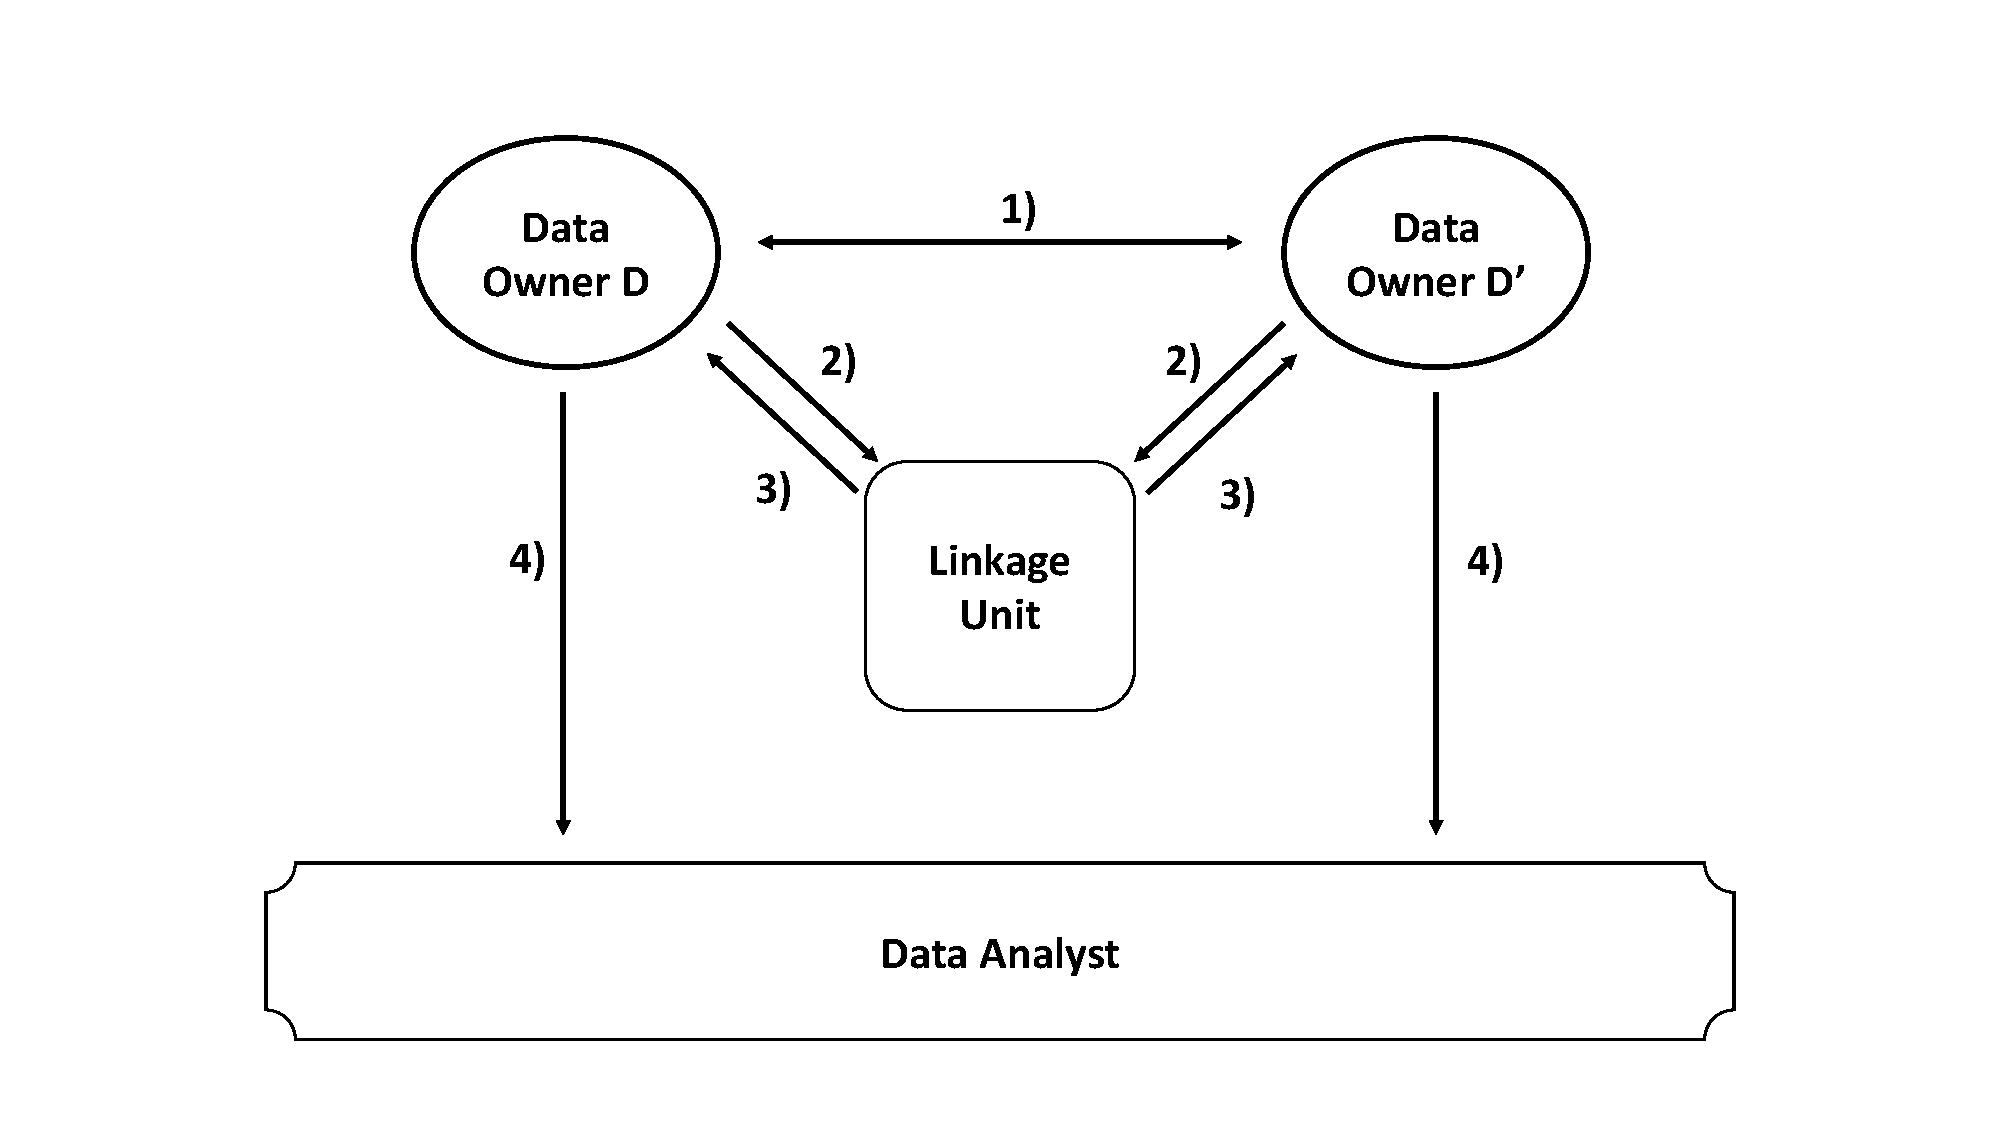
\includegraphics[width=0.6\textwidth, page=1]{img/visualization.pdf}
  \caption{Overview of the \ac{pprl} process.}
  \label{fig:pprloverview}
\end{figure}

Based on this scheme, each database record can therefore during the linkage process be represented as $r = (\lambda,  \sigma)$, where $\lambda$ denotes the linkage data which are encoded quasi-identifiers such as names and birthdates and $\sigma$ refers to the remaining microdata like in a health care scenario patient information \cite{schaefer2024}.

Linkage in \ac{pprl} is performed probabilistically, meaning that two records, \(r\) and \(r'\), are considered linked if their similarity score on \(sim(\lambda_r, \lambda_{r'})\) exceeds a predefined threshold.
The choice of threshold plays an important role in balancing the quality of the linkage.
Lower thresholds tolerate more variation and matches between records but increase the likelihood of false positives, while higher thresholds reduce false positives but may miss legitimate matches.
Thus, selecting the optimal threshold is a trade-off that requires careful consideration of the specific goals and constraints of the linkage process \cite{schaefer2024}.

A robust \ac{pprl} scheme must satisfy several important criteria to ensure effective and secure linkage.
First, a similarity function, \(sim(\lambda_r, \lambda_{r'})\), must exist to determine if two records belong to the same entity based on a predefined threshold.
Second, an encoding scheme \(enc(\lambda)\)  must be applied to \(\lambda\) in such a way that the linkage unit cannot reconstruct the original data.
Finally, a function \(sim(enc(\lambda_r), enc(\lambda_{r'}))\) must be available that allows similarity computations on encoded data.
These requirements ensure both the privacy and the effectiveness of the record linkage process \cite{schaefer2024}.

One common approach for measuring similarity for two quasi identifiers and enabling probabilistic matching on quasi identifieres is using n-grams.
Here, string values are divided into overlapping substrings of length $n$ using a sliding window approach \cite{schaefer2024}.
For example, for the string ``encoding'' with $n=2$, the n-grams are:
$$ \{\text{en}, \text{nc}, \text{co}, \text{od}, \text{di}, \text{in}, \text{ng} \} $$

The similarity of two sets of n-grams can then be computed using metrics such as the Dice Coefficient where X and Y denotes two sets which are in the case of \ac{pprl} the n-grams for two different pseudo identifiers \cite{schaefer2024}.
  $$ Dice(X, Y) = \frac{2 \cdot |X \cap Y|}{|X| + |Y|} $$
The Jaccard Similarity can be used in a similar way \cite{schaefer2024}.
  $$ Jaccard(X, Y) = \frac{|X \cap Y|}{|X \cup Y|} $$

\ac{pprl} has been successfully applied in various domains, demonstrating its practical importance in securely linking records across institutions while trying to preserve privacy.
Notable applications include the Social Investment Data Resources, the Lumos Initiative, the Swiss National Cohort, and the Gemeinsamer Bundesausschuss.
These implementations highlight the versatility of \ac{pprl} in diverse contexts, where privacy protection is essential while enabling effective data linkage for research and analysis \cite{schaefer2024}.



\section{Key Encoding Techniques} \label{sec:key-encodings}

In the context of \ac{pprl}, three primary encoding techniques have emerged: \ac{bf}, \ac{tmh} and \ac{tsh}.
These encoding methods are essential for transforming sets of quasi-identifiers into representations that preserve similarity information while trying to maintain privacy \cite{schaefer2024,vidanage2020graph, schnell2009privacy}.

\ac{pprl} typically involves encoding sets of quasi-identifiers before linkage.
A set in this context is generally a collection of n-grams, which are substrings of length $n$ extracted from one or multiple attributes using a sliding window approach.
Since input data varies in length, all encoding techniques in \ac{pprl} must take arbitrarily long inputs (sets of n-grams) and produce encoded outputs.
This ensures that similarity computations can be efficiently performed on encoded data by the linkage unit without accessing the raw identifiers \cite{vidanage2020graph,schaefer2024}.

Before linkage, data owners must agree on the encoding scheme and share necessary cryptographic secrets to facilitate secure comparison.
Among the available techniques, \ac{bf}s are the most widely used approach for record linkage \cite{schaefer2024}.

\subsection{\ac{bf}} \label{sec:bf}

\ac{bf}s were originally developed for efficient membership testing in set structures without requiring direct access to the sets themselves \cite{bloom1970space}.
Due to their ability to efficiently compute set similarities in a privacy-preserving manner, they have been widely adopted in \ac{pprl} applications \cite{schaefer2024,vidanage2020graph,schnell2009privacy}.

A \ac{bf} $b \in \{0,1\}^l$ is a bit vector of length $l$.
It uses $k \geq 1$ independent hash functions $H = \{h_1, h_2, ..., h_k\}$, where each function maps an arbitrary input to a position in the filter \cite{schaefer2024,schnell2009privacy}:
\begin{equation}
  h_i: \{0,1\}^* \to \{1, ..., l\}, \quad \forall i \in \{1, ..., k\}
\end{equation}
Initially, the \ac{bf} is set to all zeros.
Each element $s \in S$ is hashed with every function $h_i$, and the corresponding bit positions in the filter are set to 1 \cite{schaefer2024,schnell2009privacy}:
\begin{equation}
  \forall s \in S, \forall h_i \in H, \quad b[h_i(s)] = 1
\end{equation}

An Example for this can be seen in Figure~\ref{fig:bfexample} where the set of 2-grams for the word ''encoding'' is encoded using a \ac{bf} with $k = 2$ hash functions. As can be seen, the 2-grams are hashed using the two hash functions and the corresponding bits are set to 1 in the \ac{bf}.

\begin{figure}[H]
  \centering
  \includegraphics[width=0.6\textwidth, page=5]{img/visualization.pdf}
  \caption{Example \ac{bf} for $k = 2$ hash functions on the set of 2-grams for ''encoding''.}
  \label{fig:bfexample}
\end{figure}

Since \ac{bf}s are binary vectors, the similarity between two \ac{bf}s, \(b_1\) and \(b_2\), is computed based on the overlapping 1-bits based on their position.
The Dice Coefficient is commonly used for this purpose \cite{schaefer2024}, providing a measure of similarity by comparing the overlap of 1-bits in the two binary vectors.
Therefore encodings using \ac{bf} encoding allows for efficient computation of similarity between two sets which is benefical for \ac{pprl} systems.
\begin{equation}
  \text{Dice}(b_1, b_2) = \frac{2 \cdot |b_1 \cap b_2|}{|b_1| + |b_2|}
\end{equation}

Because the sets in a \ac{pprl} systems consists of n-grams, a deterministic relationship between the n-grams present in the quasi-identifier $\lambda$ and the set bits in the \ac{bf} is created.
However, due to the finite length of \ac{bf}s, collisions occur where different n-grams map to the same bit position (see Figure~\ref{fig:bfexample}).
While this can cause incorrect linkages, it also enhances privacy by distorting frequency distributions \cite{vidanage2020graph,schaefer2024}.

Three primary approaches exist for applying \ac{bf}s to sensitive data.
The first approach, Attribute-Level \ac{bf}s, encodes each attribute, such as first name or last name, into a separate \ac{bf}, enabling multiple similarity computations.
However, Attribute-Level \ac{bf}s are more vulnerable to frequency-based privacy attacks as they lower the collisions which would occur using only one \ac{bf}.
The second approach, Cryptographic Long-Term Key Encoding, merges multiple attributes into a single \ac{bf}, reducing vulnerability to frequency attacks but remaining susceptible to pattern-mining-based attacks.
Finally, Record-Level \ac{bf}s employ a weighted bit sampling technique to minimize frequency information, enhancing privacy protection while maintaining high linkage quality.
Each of these approaches balances privacy concerns with the need for accurate and effective record linkage \cite{vidanage2020graph}.

Several privacy-enhancing methods have been proposed to mitigate frequency attacks in \ac{bf}s.
These techniques introduce a trade-off between privacy and linkage quality.
One such method is balancing, which ensures an equal number of 1-bits across \ac{bf}s, thereby reducing the likelihood of frequency-based attacks.
Another approach is salting, which randomizes bit positions to prevent direct inference from the encoded quasi-identifiers.
Additionally, XOR folding is used to reduce the \ac{bf} length while maintaining the bit-wise dependencies necessary for effective linkage.
These methods aim to strengthen privacy while retaining the accuracy of the linkage process \cite{vidanage2020graph,schaefer2024}.

A major improvement was introduced by Armknecht et al. \cite{armknecht2023strengthening}, who proposed a diffusion layer for \ac{bf} encodings.
This method generates \ac{eld}, where each bit is computed as the XOR sum of multiple \ac{bf} bits.
The indices for XOR computations are randomly chosen and secretly shared among data owners \cite{armknecht2023strengthening}.

By applying diffusion, the deterministic relationship between 1-bits in the \ac{eld} and the original n-grams is broken, improving privacy while still enabling approximate matching \cite{armknecht2023strengthening}.

\ac{bf}s remain a core technique in \ac{pprl} due to their efficiency and scalability.
However, their vulnerability to frequency attacks has led to improvements such as Record-Level \ac{bf}s and diffusion layers, which enhance privacy at the cost of increased computational complexity \cite{schaefer2024, vidanage2020graph,armknecht2023strengthening}.


\subsection{\ac{tmh}} \label{sec:tmh}

\ac{tmh} is a variation of MinHash initially introduced for efficient estimation of set similarities and later adapted for privacy-preserving probabilistic record linkage.
MinHash itself was first proposed in the context of document resemblance and containment estimation.
\ac{tmh} extends MinHash by employing tabulation-based hashing, which enhances its security compared to \ac{bf}s \cite{vidanage2020graph,broder1997resemblance}.

MinHash aims to approximate the Jaccard similarity between two sets, \(S\) and \(S'\).
The fundamental idea is to represent both sets as sequences of randomly ordered elements and apply multiple rounds of random permutations \(\pi\) to shuffle them.
After each round, the first elements of both sequences are compared.
The larger the intersection between \(S\) and \(S'\), the higher the probability that the first elements will match.
An example for this can be seen in Figure~\ref{fig:minhashexample} where the sets are permutated twice and the first element is compared for each new set.
The final Jaccard similarity estimate is computed based on the number of collisions achieved during permutation, in the example is one collision for two permutations \cite{schaefer2024,broder1997resemblance,vidanage2020graph}.

\begin{figure}[H]
  \centering
  \includegraphics[width=0.6\textwidth, page=6]{img/visualization.pdf}
  \caption{Example computing approximate Jaccard similarity using MinHash with \(\pi = 2\) permutations.}
  \label{fig:minhashexample}
\end{figure}

Instead of explicitly computing these permutations, MinHash simulates them by applying a suitable hash function to the elements of a set and selecting the smallest hash value as the representative signature.
This is equivalent to sorting set elements by their hash values and returning the first element \cite{schaefer2024}.

Tabulation-based hashing is a technique used in \ac{tmh} that provides efficient and high-quality hash functions by leveraging precomputed lookup tables.
This method operates as follows \cite{vidanage2020graph}:

The process begins with the \textbf{initialization} of \(l\) sets of lookup tables, each containing \(c\) tables.
Each table holds randomly generated bit strings for keys of length \(k\), with a key space of \(2^k\).
During the \textbf{hashing process}, each element in \(S\) is hashed using a one-way hash function, producing a fixed-length binary value.
This binary value is then split into \(c\) sub-keys, each of length \(k\).
Each sub-key is used as an index to retrieve a random bit string from the corresponding lookup table, and the retrieved \(c\) bit strings are XORed together to produce a single output bit string.
In the \textbf{MinHash signature generation} phase, this process is repeated for each of the \(l\) lookup table sets, and the minimum value among all generated bit strings is selected as the MinHash signature \cite{schaefer2024,vidanage2020graph}.

An example for this can be seen in Figure~\ref{fig:tabminhashexample} where the first element of the set is hashed using the first lookup table and the fourth hash function.
The key is split into \(c = 4\) sub-keys of length \(k = 2\) and used to retrieve the corresponding bit strings from the lookup table.
The retrieved bit strings are then XORed together to produce the final value for the first element.

\begin{figure}[H]
  \centering
  \includegraphics[width=0.6\textwidth, page=7]{img/visualization.pdf}
  \caption{Simplified \ac{tmh} hasing step for the first lookup table, fourth hash function on the first set element.}
  \label{fig:tabminhashexample}
\end{figure}


To further enhance privacy, \ac{tmh} employs a 1-bit hashing mechanism, where only the least significant bit of each MinHash signature is retained.
These $l$ bits are then concatenated to form the final bit array used as an encoded representation \cite{schaefer2024}.

The main advantage of \ac{tmh} over \ac{bf}s is its improved resistance to frequency-based attacks due to the complexity introduced by tabulation-based hashing.
However, this security enhancement comes at a cost.
It leads to higher computational overhead, as the need to generate and access multiple lookup tables increases processing time.
Additionally, there is increased memory consumption because storing large precomputed tables requires additional space.
These trade-offs must be considered when choosing between \ac{tmh} and other privacy-preserving techniques \cite{schaefer2024,vidanage2020graph}.
Despite these trade-offs, \ac{tmh} remains an attractive alternative for \ac{pprl} due to its robustness against adversarial attacks.

Similar to \ac{bf}s, \ac{tmh} encodes each record as a bit vector of length $l$.
Given two \ac{tmh}-encoded bit vectors, their similarity can be estimated using a modified Jaccard coefficient, adapted to account for artificial bit collisions caused by truncation to the least significant bit.
The Jaccard coefficient can also be converted into the Dice coefficient for improved comparability with \ac{bf}-based methods \cite{vidanage2020graph,schaefer2024}.

Overall, \ac{tmh} provides a more secure encoding alternative to \ac{bf}s in \ac{pprl}, though at the expense of increased computational and memory requirements \cite{schaefer2024, vidanage2020graph}.


\subsection{\ac{tsh}} \label{sec:tsh}

\ac{tsh} is the most recent encoding scheme proposed for \ac{pprl}, introduced in 2020 \cite{ranbaduge2020secure}.
\ac{tsh} was designed to address both the privacy vulnerabilities of \ac{bf}s and the computational complexity of \ac{tmh} while maintaining accuracy in similarity calculations.
Similar to other encoding techniques, \ac{tsh} requires the input to be split into a set of n-grams $S$ prior to encoding \cite{ranbaduge2020secure}.

As a result of \ac{tsh} encoding, each record from a sensitive database is represented by a set of integers, which can be directly used to compute Jaccard similarity.
\ac{tsh} employs two distinct hashing steps.
In the first hashing step, the input set is converted into a bit matrix representation.
In the second hashing step, the bit matrix columns are mapped into integers, enabling efficient comparison.
This two-step process allows \ac{tsh} to represent sensitive data in a way that facilitates effective similarity computation while preserving privacy \cite{schaefer2024}.
These steps provide accurate Jaccard similarity calculations while improving privacy protection compared to traditional \ac{bf}-based encodings \cite{ranbaduge2020secure}.

In the first step of the \ac{tsh} process, elements of the n-gram set \(S\) are hashed into \(k\) independent \ac{bf}s \(b_i\) of length \(l\), meaning each hash function results in a corresponding bit vector.
This generates a \(k \times l\) matrix, where each row corresponds to a \ac{bf} created using a unique hash function, and each column represents the bitwise state across all \ac{bf}s for a given position.
In the second step, after constructing the bit matrix, \ac{tsh} computes column-wise hashes to convert the bit vectors into integer representations.
Each column vector is treated as an input for a hash function, and all-zero columns are skipped to prevent distortion in similarity calculations since they do not encode any n-grams.
To enhance security and avoid hash collisions between columns with identical bit patterns, a salt value and the column index are concatenated before hashing \cite{ranbaduge2020secure}.

The final integer representation for each column $i$ for $1 \leq i \leq l$. is computed as \cite{schaefer2024, ranbaduge2020secure}:
\begin{equation}
    H(salt, i, b_{1i}, b_{2i}, ..., b_{ki})
\end{equation}

The output of the second hashing step is a set of integers, allowing similarity computations using the Dice coefficient rather than directly computing bitwise similarity.
Since the encoded data consists of sets, Jaccard similarity can also be computed similarly to MinHash-based encodings \cite{ranbaduge2020secure}.

\begin{figure}[H]
  \centering
  \includegraphics[width=0.6\textwidth, page=8]{img/visualization.pdf}
  \caption{\ac{tsh} example for for two input values ''peter'' and ''pete'' \cite{ranbaduge2020secure}.}
  \label{fig:tshexample}
\end{figure}

An illustrative example is provided in Figure~\ref{fig:tshexample}, where the set of 2-grams for the words ``\textit{peter}'' and ``\textit{pete}'' is encoded using \ac{tsh} with $k = 4$ hash functions and a \ac{bf} length of $l = 8$.
In the first hashing step, each 2-gram is processed using the $k$ hash functions, resulting in a $4 \times 8$ bit matrix.
Each row of this matrix corresponds to a \ac{bf} generated with a distinct hash function, encoding the presence of 2-grams across the $l$ bit positions.

In the second hashing step, the columns of the bit matrix are transformed into integer values.
This is achieved by applying an additional hash function that incorporates both a salt value and the column index, effectively compressing the binary representation into a fixed-length integer vector.
The final output is a set of integers representing the encoded word, which can subsequently be used to compute similarity scores between different words~\cite{ranbaduge2020secure}.

To improve efficiency, \ac{tsh} can be implemented using a \ac{prng} instead of cryptographic hash functions.
The \ac{prng} is seeded with the value to be hashed before generating random numbers, ensuring that the sequence of generated values depends deterministically on the input \cite{ranbaduge2020secure}.

By combining efficient bit vector representations with integer-based similarity computations, \ac{tsh} offers a balance between privacy, security, and computational efficiency, making it a promising alternative to existing \ac{pprl} encoding schemes \cite{vidanage2020graph, ranbaduge2020secure}.

\section{\ac{gma}} \label{sec:gma}

\ac{gma}s  were introduced by Vidanage et al. \cite{vidanage2020graph} and represent the most significant threat to \ac{pprl} due to their universal applicability.
Unlike traditional cryptanalytic attacks, \ac{gma}s exploit the fundamental properties of non-interactive \ac{pprl} to compromise the security of all schemes relying on similarity-preserving encoding \cite{schaefer2024}.


Non-interactive \ac{pprl} refers to linkage schemes where data owners independently encode their data and share it with a linkage unit.
The linkage unit then performs record matching solely based on the encoded data, without requiring further interaction with the data owners during the linkage process.
This approach minimizes communication overhead and computational complexity, as no iterative exchanges between parties are necessary.
In contrast, interactive PPRL methods involve multiple rounds of communication between data owners and the linkage unit to refine matching results or improve accuracy \cite{kum2014privacy}.

In \ac{pprl}, encoded records are linked based on similarity computations.
Since these similarities serve as identifiers, an attacker with access to an encoded dataset can leverage an auxiliary plaintext dataset to re-identify individuals.
The latest version of the \ac{gma} developed by Schaefer et al. \cite{schaefer2024} overcomes the limitations of the original attack by Vidanage et al. \cite{vidanage2020graph} and enhances success rate and robustness, even under limited knowledge scenarios \cite{schaefer2024}.

In the context of a \ac{gma} on a \ac{pprl} system, the attacker is modeled as the linkage unit and is assumed to have minimal prior knowledge.
The attacker does not know any encoding secrets, seeds, or salts used in the system to protect the data.
The only information available to the attacker is that which is inevitably known to the linkage unit during the linkage process.
This assumption ensures that the attacker can only exploit data accessible through normal system operations, adhering to Kerckhoffs's principle \cite{schaefer2024}.

Since the attack does not depend on specific encoding parameters or attribute frequency distributions, it is universally applicable as long as pairwise similarities of encoded data are available \cite{schaefer2024}.

The first step of the attack involves constructing similarity graphs for both the encoded dataset (\(D_{enc}\)) and the plaintext dataset (\(D_{plain}\)).
In these graphs, each node represents an individual record, while edges between nodes are assigned weights based on pairwise similarity computations.
To ensure computational efficiency and focus only on meaningful connections, edges with similarity scores below a predefined threshold are omitted, reducing noise and improving the accuracy of the attack \cite{schaefer2024}.

Since certain encoding properties, such as \ac{bf} length ($l$), are inevitably known to the linkage unit, $D_{plain}$ can be transformed analogously to $D_{enc}$ for effective comparison.
Importantly, this step does not require knowledge of shared secrets, as the primary objective is to replicate the effect of encoding on similarity \cite{schaefer2024}.

To quantify the structural similarity between nodes in \(G_{plain}\) and \(G_{enc}\), node embeddings are computed to transform the graph structure into a numerical representation.
This process begins with graph embedding using the Node2Vec algorithm, which applies a Word2Vec-like approach to learn vector representations of nodes.
During this process, nodes undergo multiple random walks, where each walk simulates a sequence of transitions between connected nodes.
These sequences are then treated as sentences, allowing the model to learn embeddings that capture the local and global structure of the graph.
The behavior of these random walks is controlled by two hyperparameters: \(p\), which determines the likelihood of returning to a previously visited node, and \(q\), which influences the tendency to explore new regions of the graph.
The result is an embedding matrix where each row represents a node as a vector in Euclidean space \cite{schaefer2024}.

Once embeddings are generated, they must be aligned to allow meaningful comparison between the two graphs.
Due to the randomness inherent in embedding generation, direct comparison is not possible.
Instead, an iterative approach is used to solve two subproblems: first, an optimal linear transformation is determined using Procrustes Analysis to align the embeddings, and second, node correspondences are established via the Sinkhorn Algorithm, which minimizes the Wasserstein distance between the distributions of embeddings in both graphs.
To achieve an effective alignment, an unsupervised stochastic optimization scheme alternates between these two steps over \(n\) epochs, gradually refining the transformation and correspondences until convergence \cite{schaefer2024}.

Once the embeddings from the plaintext and encoded datasets are aligned, the reidentification process can begin.
Each embedding in the transformed plaintext space is compared to its counterparts in the encoded space, with similarity measured using cosine similarity.
This metric quantifies how closely two embeddings align in the high-dimensional space, enabling the attacker to identify records in the encoded dataset that most closely resemble those in the plaintext dataset \cite{schaefer2024}.

The final step involves constructing a bipartite graph, where nodes from the plaintext and encoded datasets are linked based on their similarity scores.
To determine the optimal mapping, the Jonker-Volgenant algorithm is applied, ensuring that each node in the smaller dataset is uniquely matched to a corresponding node in the larger dataset.
This algorithm maximizes the total similarity across all matched pairs, effectively revealing the identities of individuals within the encoded dataset \cite{schaefer2024}.

An example of this process is illustrated in Figures~\ref{fig:gmaexampleone} and \ref{fig:gmaexampletwo}, which provide a high-level overview of the \ac{gma} attack applied to a \ac{pprl} approach using \ac{bf} encoding.
Initially, the two data owners agree on an encoding scheme and encode their respective datasets, for this example using \ac{bf}.
These encoded datasets are then send to the linkage unit.
The attack begins at this point, leveraging information inherently available to the linkage unit.
Specifically, the linkage unit constructs similarity graphs for both the encoded datasets and an auxiliary plaintext dataset.
By embedding these similarity graphs into a vector space and aligning the embeddings, the attacker can identify re-identifications by comparing embeddings and constructing a bipartite graph that matches entries from the encoded dataset to those in the plaintext auxiliary dataset \cite{schaefer2024}.


\begin{figure}[H]
  \centering
  \includegraphics[width=0.6\textwidth, page=10]{img/visualization.pdf}
  \caption{High-level overview of the \ac{gma} attack process.
  Two data owners encode their datasets and send them to the linkage unit.}
  \label{fig:gmaexampleone}
\end{figure}

\begin{figure}[H]
  \centering
  \includegraphics[width=0.6\textwidth, page=11]{img/visualization.pdf}
  \caption{High-level overview of the \ac{gma} attack process.
  The linkage unit mimics the \ac{bf} encoding for the public dataset and creates for both datasets similartie graphs, embeddings and aligns them to perform bipartite matching.}
  \label{fig:gmaexampletwo}
\end{figure}

The improved \ac{gma} approach by Schaefer et al. \cite{schaefer2024} achieves near-perfect re-identification rates when dataset overlap is 100\%.
Even for low-overlap scenarios (e.g., 5\%), success rates reach 99.9\% for \ac{tsh} \cite{schaefer2024}.
The only encoding scheme resistant to \ac{gma}s is \ac{bf}s with diffusion layers, which disrupts similarity preservation for sufficiently high diffusion values \cite{schaefer2024}.


\section{\ac{ann}} \label{sec:nn}

\ac{ann}s are a class of \ac{ml} models inspired by the structure and function of biological neural systems.
They consist of interconnected layers of artificial neurons that process input data and extract meaningful patterns through iterative learning.
\ac{ann}s have been widely applied in various fields, including image recognition, natural language processing, and classification tasks.
Neural networks are particularly effective for complex tasks because they automatically identify and refine patterns in data through multiple layers of processing, removing the need for manual feature engineering, which can be difficult and time-consuming \cite{dongare2012introduction}.

The structure of an \ac{ann} consists of multiple layers as can be seen in Figure~\ref{fig:annexample}, each serving a distinct role in processing and transforming input data.
The input layer is the first stage of the network, responsible for receiving raw data and forwarding it to subsequent layers.
The number of neurons in this layer corresponds directly to the number of input features, ensuring that all relevant information is passed through the network \cite{dongare2012introduction, sharma2024deep}.

\begin{figure}[H]
  \centering
  \includegraphics[width=0.4\textwidth, page=16]{img/visualization.pdf}
  \caption{\ac{ann} consisting of multiple input neurons (input layer), hidden layers and output neurons (output layer) \cite{annimage}.}
  \label{fig:annexample}
\end{figure}


Following the input layer are the hidden layers, which perform feature extraction and transformation.
Each neuron in a layer applies a weighted sum operation to its inputs, followed by an activation function that introduces non-linearity, enabling the network to learn complex patterns in the data. Common activation functions include the Rectified Linear Unit (ReLU), Sigmoid, Leaky ReLU, and Exponential Linear Unit (ELU), each offering advantages depending on the specific task \cite{sharma2017activation,russell2016artificial}.

\begin{figure}[H]
  \centering
  \includegraphics[width=0.4\textwidth, page=17]{img/visualization.pdf}
  \caption{Sketch of an single artifical neuron in an \ac{ann} \cite{neuronimage}.}
  \label{fig:neuronexample}
\end{figure}

An example of this process is illustrated in Figure~\ref{fig:neuronexample}, which depicts a single neuron in an \ac{ann}.
The neuron takes multiple inputs, multiplies them by corresponding weights, sums the weighted inputs along with a bias term, and applies an activation function to compute the final output.
Mathematically, this operation is represented as

\begin{equation}
  a = \sigma(z) = \sigma\left(\sum_{i=1}^{n} w_i x_i + b\right)
\end{equation}

where \(a\) is the neuron’s output, \(\sigma\) is the activation function, \(z\) is the weighted sum, \(w_i\) are the weights, \(x_i\) are the inputs, and \(b\) is the bias term \cite{neuronimage}.
The depth and size of the hidden layers determine the network's capacity to model relationships, making them an important component of deep learning architectures \cite{dongare2012introduction, sharma2024deep}.

Finally, the output layer generates the final predictions based on the processed information.
The number of neurons in this layer depends on the nature of the task, whether it is a classification problem, where each neuron represents a class, or a regression task, where a single neuron outputs a continuous value \cite{dongare2012introduction}.

Training an \ac{ann} involves iteratively adjusting its parameters, using a labeled dataset to minimize prediction errors.
The process begins with forward propagation, where input data flows through the network, passing through multiple layers until it reaches the output layer, generating a prediction.
This prediction is then compared to the actual target value, and the discrepancy between the two is quantified using a loss function, which measures the model's performance \cite{russell2016artificial}.

To improve accuracy, the network undergoes backward propagation (backpropagation), where the gradient of the loss with respect to each weight is computed using the chain rule of differentiation.
These gradients indicate how each parameter should be adjusted to reduce the overall error \cite{russell2016artificial}.

An optimizer, such as Stochastic Gradient Descent (SGD) or Adam, updates the weights accordingly by taking small steps in the direction that minimizes the loss.
The training process is repeated over multiple epochs, where the entire dataset is processed multiple times.
To enhance efficiency, the data is often divided into batches, allowing the model to update its weights incrementally rather than processing the entire dataset at once.
Over time, this iterative optimization process enables the network to learn meaningful patterns and improve its predictive performance.
\ac{ann}s can be applied to different classification tasks, depending on whether a data instance belongs to a single category or multiple categories simultaneously \cite{russell2016artificial}.

In traditional single-label or binary classification problems, each instance is assigned to one and only one category from a predefined set of classes.
To achieve this, the network's output layer typically uses a Softmax activation function, which converts the raw output scores into a probability distribution over all possible classes.
The model can be trained using the Cross-Entropy Loss function, which penalizes incorrect classifications by measuring the difference between the predicted probability distribution and the actual class label \cite{russell2016artificial,herrera2016multilabel}.

In contrast, multi-label classification allows an instance to belong to multiple categories (labels) at the same time.
Instead of a single categorical output, the network produces independent predictions for each possible label.
The output layer can then as an example apply sigmoid activations for each label, transforming the raw scores into independent probabilities indicating the presence or absence of each class.
Since each label is treated as a separate binary classification problem, Binary Cross-Entropy (BCE) Loss is commonly used to optimize the model, ensuring accurate predictions across multiple labels \cite{russell2016artificial,herrera2016multilabel}.

Different \ac{ann} architectures have been developed to address various problem domains, each optimized for specific types of data and tasks.
Feedforward \ac{ann}s (FNNs) represent the simplest architecture, where data flows in one direction from the input layer to the output layer without forming cycles.
These networks are widely used for basic classification and regression tasks but may struggle with complex patterns that require spatial or sequential dependencies \cite{russell2016artificial,glorot2010understanding}.

For tasks involving image processing, Convolutional \ac{ann}s (CNNs) are commonly used.
CNNs employ convolutional layers that apply filters to input images, allowing the network to capture complex patterns such as edges, textures, and shapes.
This makes them highly effective for applications like object recognition and medical imaging \cite{o2015introduction, sharma2024deep}.

When dealing with sequential data, Recurrent \ac{ann}s (RNNs) and their advanced variant, Long Short-Term Memory (LSTM) Networks, are particularly useful.
These architectures introduce recurrent connections, enabling them to maintain memory of previous inputs and recognize patterns over time.
This makes them well-suited for natural language processing, speech recognition, and time series forecasting \cite{medsker2001recurrent}.

Despite their success, \ac{ann}s present several challenges that must be managed to ensure robust and efficient learning.
One of the most common issues is overfitting, where a model becomes too specialized in learning patterns from the training data, capturing possible noise rather than generalizable features.
This leads to poor performance on unseen data.
Techniques such as dropout regularization, L2 weight decay, and early stopping are commonly used to mitigate overfitting and improve generalization \cite{pytorchPyTorch,glorot2010understanding}.

Dropout regularization is a technique used to prevent overfitting by randomly setting a fraction of neurons to zero during training.
This forces the network to learn more robust features by preventing it to rely too heavily on a single neuron to perform well.
L2 weight decay is another regularization method that penalizes large weights by adding a regularization term to the loss function.
It tries to prevent the network from applying too much importance to a single feature, encouraging it to learn more generalizable patterns.
Early stopping is a simple yet effective technique that stops training when the model's performance on a validation set starts to degrade below a certain threshhold, preventing overfitting \cite{pytorchPyTorch,glorot2010understanding}.

Another fundamental challenge is the vanishing and exploding gradient problem, which occurs in deep networks during backpropagation.
When gradients become too small (vanishing), weight updates diminish, leading to slow or stalled learning.
This can happen because gradients are the product of multiple derivatives, which can cause them to shrink exponentially as they propagate through the network.
This can happen especially using activiation functions that saturate for extreme values.
Conversely, when gradients grow too large (exploding), unstable updates cause erratic training behavior.
Solutions such as batch normalization, gradient clipping, and advanced activation functions like Leaky ReLU help address these issues \cite{pytorchPyTorch,glorot2010understanding}.

Batch normalization stabilizes training by normalizing the inputs to each layer, ensuring that activation values remain within a consistent range.
Gradient clipping addresses the problem of exploding gradients by imposing a threshold on gradient values, thereby maintaining training stability.
Leaky ReLU, an activation function, mitigates the vanishing gradient problem by allowing a small, non-zero gradient for negative inputs, enabling continued learning even with extreme input values \cite{pytorchPyTorch,glorot2010understanding}.

The computational complexity of deep learning models is another major concern, as large-scale \ac{ann}s require extensive memory and processing power.
Training deep networks on large datasets can be prohibitively slow on CPUs, necessitating the use of GPUs or specialized hardware like TPUs (Tensor Processing Units) to accelerate training.
Efficient data-loading techniques and mixed-precision training can further optimize computational efficiency.
Mixed-precision training is a technique that partly uses lower-precision floating-point numbers to reduce memory usage and speed up computations, while still maintaining model accuracy \cite{pytorchPyTorch}.

Lastly, hyperparameter tuning plays an important role in model performance.
Selecting the right learning rate, batch size, number of layers, and optimization algorithm requires experimentation and fine-tuning.
Automated methods such as grid search, random search, and Bayesian optimization can assist in finding optimal configurations, but these processes are computationally expensive.
Addressing these challenges effectively is important for developing high-performing \ac{ann}s that generalize well across different datasets and tasks \cite{pytorchPyTorch}.

   %% The background chapter
\chapter{Methodology}  \label{sec:method}
The \ac{dea} is a novel attack method that extends the capabilities of \ac{gma}s by moving beyond the intersection of datasets to re-identify individuals who were previously unmapped.
This chapter outlines the methodology behind the \ac{dea}, including modifications to the \ac{gma}, the design and implementation of the \ac{dea} itself, and the use of \ac{ann}s to enable probabilistic reconstruction of \ac{pii} from encoded data.

The \ac{dea} builds upon the \ac{gma} by using its re-identification results as a foundation for further inference.
While the \ac{gma} re-identifies only those records that exist in both the attacker’s dataset and the encoded target dataset, it often leaves a substantial portion of records unmapped.
The goal of the \ac{dea} is to extend this re-identification process by applying a machine learning–based approach to infer the missing \ac{pii} of the remaining records using a trained \ac{ann}.

To achieve this, the \ac{dea} follows a structured pipeline comprising several key steps, as illustrated in Figure~\ref{fig:deaoverview}.
First, the results of the \ac{gma} are extracted in a predefined format to serve as training data for the \ac{ann}.
These results include the re-identified individuals, their corresponding encoded representations, and the plaintext information that was successfully mapped.
In addition, the \ac{gma} results contain the non-re-identified individuals, represented only by their encoded \ac{pii} and plaintext information.
Maintaining a consistent and structured format is essential to ensure seamless integration into subsequent processing stages.

\begin{figure}[H]
    \centering
    \includegraphics[width=0.7\textwidth, page=14]{img/visualization.pdf}
    \caption{Overview of the \ac{dea} attack pipeline.}
    \label{fig:deaoverview}
  \end{figure}

Once the data is extracted, it is transformed into a format suitable for \ac{ann} training.
This involves constructing specialized datasets that convert encoded representations and their corresponding labels—plaintext n-grams—into tensor-based formats that can be efficiently processed by deep learning models.
The datasets are then split into training, validation, and test sets, and corresponding data loaders are created to enable efficient batch processing during training.

With the data pipeline in place, an \ac{ann} is designed to perform multi-label classification, predicting the likelihood of individual n-grams occurring in an encoded record.
The architecture comprises an input layer that receives the encoded representation, a series of hidden layers that learn complex patterns in the data, and an output layer that generates probability scores for all possible n-grams.

To optimize performance, an appropriate loss function, optimizer, and learning rate scheduler must be selected to ensure stable convergence and high predictive accuracy.
To this end, a hyperparameter optimization is performed, in which various configurations are systematically evaluated to identify the best-performing model.
The final model, with the optimal configuration, is then trained on the training set, while performance is monitored on the validation set to prevent overfitting.

Once the \ac{ann} is trained, it can be applied to the set of non-re-identified individuals, i.e., records that remained unmapped after the \ac{gma}.
This dataset serves as the test set during the experimentation phase to evaluate the performance of the attack.

The model outputs a probability distribution over all possible n-grams for each entry, indicating the likelihood of each n-gram being present in the corresponding plaintext data.
To refine these predictions, a thresholding mechanism is applied to filter out low-confidence outputs and retain only the most probable n-grams.
These predicted n-grams are then aggregated and reconstructed into potential \ac{pii}, constituting the final step of the \ac{dea} process.

This methodological approach represents a significant advancement in attacking \ac{pprl} systems.
By leveraging deep learning techniques, the \ac{dea} enables an attacker to infer sensitive personal information beyond the scope of traditional \ac{gma} approaches.
The following sections provide a detailed discussion of each component, including the design choices, implementation details, and challenges encountered during development.

\section{Modifications to the \ac{gma}} \label{sec:modifications}

The \ac{gma} serves as the foundation for the \ac{dea} by providing an initial set of re-identified individuals, including their corresponding encodings, as well as the remaining non-re-identified individuals.

The effectiveness of the \ac{dea} is directly influenced by the performance of the \ac{gma}.
A higher re-identification rate in the \ac{gma} yields a larger training dataset for the \ac{dea}, thereby enhancing its ability to infer n-grams and re-identify individuals in the non-re-identified dataset.
Conversely, a low re-identification rate limits the availability of labeled training data, reducing the overall effectiveness of the \ac{dea}.

To integrate the \ac{gma} as a preprocessing step for the \ac{dea}, modifications were made to the original implementation by Schaefer et al.~\cite{schaefer2024}.
While the core algorithm remains unchanged, adjustments were introduced to ensure that the \ac{gma} outputs its results in a structured format suitable for training the \ac{ann} used in the \ac{dea}.

Originally, the \ac{gma} only provided a simple mapping between the IDs of re-identified individuals.
However, to enable the \ac{dea} to learn meaningful patterns, access to both the plaintext \ac{pii} and their corresponding encodings is required.
Therefore, the \ac{gma} was extended to output two datasets in the following format:

\begin{itemize}
    \item For re-identified individuals: \texttt{<\ac{pii}> <encoding> <uid>}
    \item For non-re-identified individuals: \texttt{<encoding> <uid>}
\end{itemize}

It is important to note that the \texttt{uid} is included solely for research and evaluation purposes.
It enables researchers to manually track individuals across different processing stages and to assess the performance of the attack.
However, in a real-world attack scenario, these \texttt{uid}s are neither available nor required.
They are entirely excluded from all \ac{dea} training and inference steps, ensuring that the attack methodology remains realistic and practically applicable.

In addition to formatting adjustments, certain components of the \ac{gma} were removed to streamline the process and reduce unnecessary complexity.
Specifically, encoding schemes other than \ac{tsh}, \ac{tmh}, and \ac{bf} were excluded, as the \ac{dea} focuses exclusively on these techniques.
Other components deemed non-essential — such as graph visualizations and benchmark tests related solely to the \ac{gma} — were also removed.
This decision was made because the \ac{gma} is not the primary focus of this study; its validity and performance have already been established by prior research.
These optimizations resulted in a leaner and more efficient attack pipeline, reducing computational overhead while preserving essential functionality.

With these modifications in place, the starting point for the \ac{dea} is clearly defined.
The attack begins with two structured datasets:

\begin{enumerate}
    \item Re-identified individuals, containing both plaintext \ac{pii} and corresponding encodings, formatted as described above.
    \item Non-re-identified individuals, for whom only the encodings are available, serving as the primary targets for inference using the \ac{dea}.
\end{enumerate}

By leveraging this structured output, the \ac{dea} can train a machine learning model to probabilistically reconstruct missing n-grams from the encoded records of non-re-identified individuals.
The following sections detail the implementation of this approach, including dataset preparation, model architecture, and evaluation strategies.

\section{Design and Implementation of the \ac{dea}} \label{sec:designandimplementation}

The \ac{dea} aims to reconstruct plaintext \ac{pii} from encoded records using machine learning techniques.
This section outlines the problem definition, data representation, \ac{ann} architecture, and training methodology.
A central challenge in implementing the \ac{dea} lies in the diversity of encoding schemes used to protect sensitive data.
As each encoding method transforms plaintext into distinct numerical representations, the \ac{dea} must adapt both the dataset structure and the \ac{ann} architecture accordingly.

To address this, the \ac{dea} adopts a modular design: while the overall attack methodology remains consistent, specific implementations are tailored to each encoding scheme.
Although the input representation and network architecture vary depending on the encoding, the output format is kept uniform across all models.
The attack is framed as a multi-label classification task, where the \ac{ann} predicts the likelihood of individual n-grams appearing in the original \ac{pii}.
For each encoding scheme, a dedicated dataset structure transforms encoded records into a format suitable for \ac{ann} training.
Moreover, a custom \ac{ann} architecture is employed for each encoding scheme to ensure the model effectively learns the mapping from encoded data to plaintext n-grams.


\subsection{Problem Definition} \label{sec:problemdefinition}

The primary challenge that the \ac{dea} seeks to address is the limited scope of re-identifications achieved by the \ac{gma}.
While the \ac{gma} effectively links records by exploiting structural relationships within encoded datasets, its success is inherently restricted to individuals who are present in both the plaintext and the encoded datasets and can be matched based on graph similarity.
However, in real-world scenarios, there may exist additional re-identification potential beyond these direct matches.

One possible way to extend re-identifications is to rerun the \ac{gma} iteratively, incorporating additional publicly available data to gradually refine the matching process.
However, this approach is inherently dependent on the availability and quality of external data sources, which may not always be feasible.
Instead, the \ac{dea} introduces a novel strategy that aims to reconstruct deterministic relationships between encoded representations and their corresponding plaintext information.
This is based on the observation that all encoding schemes used in \ac{pprl} rely on hash functions or other deterministic mappings.

Hash functions, for example, produce fixed-length outputs from inputs of arbitrary length and, crucially, are deterministic — meaning the same input will always yield the same output.
The \ac{dea} leverages this property by training \ac{ann}s to learn statistical relationships between encoded values and the original n-grams of \ac{pii}.
The objective is to recover the most probable plaintext representation given an encoded input, effectively framing the attack as a probabilistic, frequency-based inference problem.
However, several challenges complicate this task.

The first major challenge is the lack of knowledge about the specific number and type of hash functions used during encoding.
As a result, the model must learn patterns in the data without any explicit understanding of the underlying hashing mechanisms.
Fortunately, this limitation is partially mitigated by the fact that the \ac{dea} does not rely on a one-to-one mapping between hash outputs and plaintext n-grams, but instead depends on statistical inference across large numbers of training samples.

A more fundamental challenge arises from the collision property of hash functions.
Because hash functions map an infinite input space to a finite output space, different inputs may produce identical hash values, making it inherently difficult to perfectly recover the original plaintext.
These collisions introduce uncertainty into the re-identification process, preventing the \ac{dea} from achieving perfect reconstruction accuracy.
Consequently, the predictions made by the \ac{dea} are probabilistic rather than deterministic — it can estimate the likelihood of a specific n-gram being present in the original \ac{pii}, but cannot guarantee absolute correctness.

The primary reason the \ac{gma} alone is unable to achieve such probabilistic reconstruction is that it relies solely on structural similarities within the dataset, without attempting to infer direct relationships between encoded values and their plaintext equivalents.
In contrast, the \ac{dea} enhances the capabilities of the \ac{gma} by enabling the reconstruction of individual plaintext components directly from encoded representations, thereby increasing the overall re-identification potential.
This novel approach significantly improves the effectiveness of the attack, allowing for the re-identification of individuals who were previously unmatchable using traditional graph-based techniques.

\subsection{Data Representation} \label{sec:representation}

For an \ac{ann} to operate effectively, the input data must be preprocessed into a format compatible with deep learning models.
This preprocessing step applies to both the input — encoded representations of \ac{pii} — and the output, which consists of labels representing the predicted n-grams.
Since \ac{ann}s in PyTorch operate on tensor-based representations, the transformation of encoded records into tensors is a fundamental requirement.
This ensures that both re-identified and not-reidentified individuals are structured in a way that enables efficient training and inference.

To facilitate this transformation, custom PyTorch datasets are implemented.
These datasets convert encoded representations into input tensors and encode the corresponding n-gram labels in a multi-label classification format, where each n-gram is represented as a binary indicator within a fixed-size label vector.
This approach enables the model to predict the presence of multiple n-grams per encoded record.

The data representation pipeline is modular and accommodates various encoding schemes, each of which necessitates a tailored preprocessing technique.
Depending on the encoding method — such as \ac{bf}, \ac{tsh}, or \ac{tmh} — different strategies are employed to convert the encoded input into tensors while preserving as much discriminative information as possible.
This ensures that the input is well-suited to the architecture of the corresponding \ac{ann} and that the model can effectively learn the mapping between encoded data and plaintext n-grams.

\subsubsection{\ac{bf} Encoding}

\ac{bf}'s are fixed-length binary strings, with their length determined by Alice’s chosen encoding parameters.
The transformation of a \ac{bf} into a PyTorch tensor is straightforward: each bit in the binary string is directly mapped to a corresponding position in the tensor.
This conversion preserves the positions of set bits (i.e., ones), thereby maintaining the structural integrity of the original encoding.
The resulting tensor has the same dimensionality as the \ac{bf}, with ones indicating the activated hash positions and zeros elsewhere.
This binary representation serves as the input to the \ac{ann}, allowing the model to learn patterns based on the bitwise structure of the encoded \ac{pii}.

\subsubsection{\ac{tmh} Encoding}

\ac{tmh}, like \acp{bf}, produces fixed-length binary bitstrings, with the specific length determined by the encoding parameters selected by Alice.
The transformation into a PyTorch tensor mirrors that of the \ac{bf}: each bit in the \ac{tmh} string is mapped directly to a corresponding tensor position, preserving the locations of set bits.
This direct conversion results in a binary tensor representation that retains the structure of the original \ac{tmh} encoding.
By preserving the positional information of the activated bits, the \ac{ann} can effectively learn from the encoded patterns embedded in the \ac{tmh} representations.

\subsubsection{\ac{tsh} Encoding}

The preprocessing of \ac{tsh} encodings is more complex due to its variable-length representation.
Unlike \ac{bf} and \ac{tmh}, which produce fixed-length binary bitstrings, \ac{tsh} generates a set of integers of arbitrary size.
This variability arises because columns containing only zero values are dropped during the \ac{tsh} encoding process.

Since \acp{ann} require fixed-length input vectors, a suitable transformation must be applied to standardize \ac{tsh} encodings.
Aggregation techniques, such as computing averages, would result in significant information loss, especially this already limited knowledge setting.
Therefore, an alternative approach is employed to convert \ac{tsh} encodings into a tensor-compatible format.

To achieve this, all unique integer values from both the re-identified and non-reidentified datasets are collected and stored in a set.
This set is then sorted in ascending order and transformed into a dictionary that maps each integer to a unique index.
Using this mapping, each \ac{tsh} encoding is converted into a binary vector using a one-hot encoding scheme.
For each integer present in the \ac{tsh} encoding, the corresponding index in the binary vector is set to one, while all other positions remain zero.

Regardless of the encoding scheme used as input, the output of the \ac{ann} remains consistent across all implementations.
The model is trained to map the encoded input to a probability distribution over possible n-grams.
Thus, the output layer of the \ac{ann} performs multi-label classification, predicting the likelihood of each n-gram being present in the original plaintext \ac{pii}.

\subsection{Re-Identified Individuals as Labeled Training Data}

To enable supervised learning, re-identified individuals are used as labeled training and validation data.
Since their \ac{pii} is known along with their corresponding encoded representation, it is possible to construct datasets where the input consists of transformed encodings (\ac{bf}, \ac{tmh}, or \ac{tsh}, respectively) and the output labels consist of the correct n-grams derived from the original \ac{pii}.

To facilitate this process, a predefined dictionary of all possible n-grams is created. This dictionary includes:
\begin{itemize}
   \item Alphabetical n-grams (e.g., for 2-grams: \texttt{aa} to \texttt{zz}),
   \item Numerical n-grams (e.g., for 2-grams: \texttt{00} to \texttt{99}),
   \item Alphanumeric mixed n-grams (e.g., for 2-grams: \texttt{a0} to \texttt{z9}).
\end{itemize}

Since the datasets used in this research primarily contain first names, last names, and birthdates, these character sets are sufficient to cover the vast majority of n-gram occurrences.
Each possible n-gram is mapped to a specific index in the output tensor based on the dictionary, ensuring a consistent label format across all training samples.
For example, if index \texttt{1} corresponds to the 2-gram \enquote{ab}, and the \ac{ann} predicts a 60\% probability at index \texttt{1}, this is interpreted as a 60\% likelihood that \enquote{ab} was present in the original plaintext.

By structuring the data in this way, the \ac{ann} is trained to learn a mapping from encoded inputs to their corresponding n-gram distributions, enabling the \ac{dea} to probabilistically reconstruct plaintext \ac{pii} from encoded data.


\subsection{\ac{ann} Architecture for \ac{dea}} \label{sec:architecture}

Attempting to reconstruct plaintext information from encoded representations based on hash functions presents a significant challenge due to the nature of cryptographic hashing.
Since hash functions are designed as one-way functions, reversing the transformation to recover the original input is theoretically infeasible.
However, while exact reconstruction is not possible, a probabilistic approach can still be employed to infer likely plaintext components based on statistical patterns within the encoded data.

\ac{ann}s provide a powerful framework for learning complex mappings between input encodings and output predictions, making them well-suited for this task.
The function of the \ac{ann} in the context of the \ac{dea} is to predict n-grams by learning from re-identified individuals — those whose plaintext information is known alongside their corresponding encodings.
Through this supervised learning process, the model captures frequency patterns that emerge due to the deterministic nature of the encoding process.
In essence, the \ac{ann} learns which n-grams are statistically associated with specific positions or patterns in the encoded representations and leverages these associations to estimate their likelihood in unseen encoded inputs.

Although hash functions introduce collisions, where different inputs may produce the same hash output, the \ac{ann} can still extract meaningful probabilistic insights by generalizing over these mappings across many samples.
This enables the \ac{dea} to output a ranked list of likely n-grams per record, thereby forming the basis for the reconstruction of \ac{pii} from encoded data in a probabilistic, frequency-informed manner.


\subsubsection{General \ac{ann} Architecture}

To support the task of reconstructing n-grams from encoded data, a flexible \ac{ann} architecture is employed across all models.
This architecture is designed to adapt to the different input formats arising from various privacy-preserving encoding schemes.
Although the input representation differs depending on the encoding used, the output layer remains the same across all trained models.
The output is a probability distribution over a fixed dictionary of n-grams, where each output neuron corresponds to the likelihood of a specific n-gram being part of the original plaintext string.

The architecture follows a feedforward design and consists of three main components: an input layer, a configurable sequence of hidden layers, and a final output layer.
The size of the input layer is determined by the dimensionality of the encoded record.
For instance, in the case of the \ac{bf} and \ac{tmh} model, the input layer corresponds to the length of the bitstring, which in turn is defined by Alice’s chosen parameters.
The \ac{tsh} models define their input layers based on the number of unique integers used across both datasets.

This modular architecture enables experimentation across different encoding schemes while maintaining a unified framework for training and evaluation.

The hidden layers are structured dynamically, depending on a set of tunable hyperparameters.
These include the number of hidden layers, the number of neurons in each layer (hidden layer size), the activation function (e.g., ReLU, Tanh), and the dropout rate used for regularization.
Each hidden layer is followed by a non-linear activation function, enabling the model to capture complex and non-linear relationships in the data.
To mitigate overfitting, dropout is applied after each activation layer, randomly deactivating a fraction of neurons during training.
This regularization technique improves the model's ability to generalize to unseen inputs and prevents the memorization of training data.

The output layer remains consistent across all encoding schemes and has a dimensionality equal to the size of the predefined n-gram dictionary.
Each output neuron represents the model's predicted probability that a specific n-gram appears in the original plaintext record.
Given that multiple n-grams may be present in a single encoded record, the task is framed as a multi-label classification problem.
Therefore, the output layer uses a sigmoid activation function, allowing the network to assign independent probability estimates to each n-gram.

This modular architecture is implemented using PyTorch's \texttt{nn.Sequential} API, which enables a clean, maintainable, and extensible model definition.
Furthermore, this design supports efficient hyperparameter optimization, as critical components—such as the number of layers, hidden layer size, activation function, and dropout rate—can be systematically varied across experimental runs.
By exploring this hyperparameter space, the model can be tailored to maximize reconstruction performance for each specific encoding scheme.


\subsubsection{Hyperparameter Optimization}

Hyperparameter tuning plays a crucial role in achieving optimal model performance.
Unlike model parameters that are learned during training (e.g., weights and biases), hyperparameters are defined prior to training and control the structure of the model as well as aspects of the learning algorithm.
These include architectural choices such as the number of layers as well as training configurations like the learning rate, optimizer, and regularization techniques.
Careful selection of these values is especially important in complex tasks such as reconstructing plaintext n-grams from encoded representations, where both underfitting and overfitting can lead to substantial performance degradation.

To explore the extensive hyperparameter space efficiently, this work employs Ray Tune, a scalable library for distributed hyperparameter tuning.
Specifically, the Optuna search algorithm is used within Ray Tune to guide the optimization process.
Optuna leverages a Tree-structured Parzen Estimator, a Bayesian optimization method that prioritizes promising regions of the search space based on previous trial results.
This approach improves search efficiency and reduces the number of iterations required to discover high-performing configurations.

The hyperparameter search space in this study is designed to be both comprehensive and computationally feasible.
Key hyperparameters that define the neural network architecture include:

\begin{itemize}
    \item \textbf{Number of hidden layers} (\texttt{num\_layers}): varied between 1 and 7, allowing the exploration of both shallow and deep networks.
    \item \textbf{Hidden layer size} (\texttt{hidden\_layer\_size}): selected from \{64, 128, 256, 512, 1024, 2048\}, enabling experiments with compact to large-capacity models.
    \item \textbf{Dropout rate} (\texttt{dropout\_rate}): sampled uniformly between 0.1 and 0.4 to promote generalization and mitigate overfitting.
    \item \textbf{Activation function} (\texttt{activation\_fn}): treated as a categorical variable with options including \texttt{ReLU}, \texttt{Leaky ReLU}, \texttt{GELU}, \texttt{ELU}, \texttt{SELU}, and \texttt{Tanh}.
\end{itemize}

These architectural parameters create a flexible and expressive search space for discovering well-performing network structures tailored to the task of the \ac{dea}.

The optimization strategy is similarly governed by several hyperparameters that influence how the model is trained.
The \textbf{optimizer} is treated as a categorical hyperparameter, with options including \texttt{Adam}, \texttt{AdamW}, \texttt{RMSprop}, and \texttt{SGD}.
Each optimizer is paired with a corresponding learning rate sampled from a log-uniform distribution to accommodate the wide sensitivity of models to this parameter.
In the specific case of \texttt{SGD}, an additional \texttt{momentum} parameter is also tuned to control the influence of past gradients in the current weight update.

In conjunction with the optimizer, the choice of a \textbf{learning rate scheduler} (\texttt{lr\_scheduler}) further enhances the model's ability to converge effectively.
The search space for learning rate scheduling strategies includes:
\begin{itemize}
    \item \texttt{StepLR}: reduces the learning rate at fixed epoch intervals,
    \item \texttt{ExponentialLR}: applies exponential decay over time,
    \item \texttt{ReduceLROnPlateau}: reacts to stagnation in validation loss,
    \item \texttt{CosineAnnealingLR}: follows a cosine decay schedule,
    \item \texttt{CyclicLR}: oscillates between lower and upper bounds in modes such as \texttt{triangular}, \texttt{triangular2}, and \texttt{exp\_range}.
\end{itemize}
An additional option to disable learning rate scheduling is also included to assess whether constant learning rates perform better for certain models.

Furthermore, the \textbf{loss function} (\texttt{loss\_fn}) is a critical hyperparameter, as it directly influences the optimization objective.
Several loss functions suitable for multi-label classification are explored:
\begin{itemize}
    \item \texttt{BCEWithLogitsLoss}: a standard binary cross-entropy loss combined with a sigmoid activation,
    \item \texttt{WeightedBCE}: a weighted variant to address class imbalance,
    \item \texttt{MultiLabelSoftMarginLoss}: supports probabilistic multi-label targets,
    \item \texttt{FocalLoss}: down-weights easy examples to focus learning on hard-to-predict samples, particularly effective in imbalanced scenarios.
\end{itemize}

This comprehensive optimization configuration enables systematic exploration of training dynamics, ensuring the neural network can effectively learn meaningful mappings for the Dataset Extension Attack across various encoding schemes.

\textbf{Additional parameters} are also incorporated into the hyperparameter search to fine-tune the model's output behavior and ensure consistent evaluation.
A tunable \textbf{threshold} parameter is introduced, ranging between 0.3 and 0.8, which is used to convert the model's output probabilities into binary predictions for the presence of specific n-grams.
This threshold is particularly relevant in multi-label classification settings where choosing an appropriate cutoff directly impacts precision and recall.

The dimensions of the input and output layers, denoted by \texttt{input\_dim} and \texttt{output\_dim}, are fixed for each encoding scheme.
The \texttt{input\_dim} reflects the length of the encoded bitstring or vector depending on the method used (e.g., \ac{bf}, \ac{tmh}, or \ac{tsh}), while the \texttt{output\_dim} corresponds to the size of the n-gram dictionary, representing the total number of possible n-grams to be predicted.

To ensure a fair and consistent comparison across all hyperparameter configurations, the same \texttt{data\_train} and \texttt{data\_val} datasets are used in each trial.
This controlled setup ensures that variations in performance can be attributed to the model configuration rather than differences in training and validation data.

During tuning, Ray Tune orchestrates multiple parallel trials, each corresponding to a unique combination of hyperparameters sampled from the search space.
Optuna's pruning mechanism is also integrated, allowing unpromising trials to be stopped early based on intermediate results (e.g., validation loss), which improves overall efficiency.
Performance is evaluated on the validation set, and the best configuration is selected based on a predefined objective function.

This automated, systematic tuning process ensures that the neural network architecture is well-adapted to the complexity and characteristics of the input encoding.
It enables fair comparison across models (\ac{bf}, \ac{tmh}, or \ac{tsh}) and improves both the predictive performance and generalization capability of the reconstruction task.

\subsection{Training the Model} \label{sec:training}

To effectively train and evaluate the \ac{ann} model with the best hyperparameters, the dataset is divided into three distinct subsets: a training set, a validation set, and a test set.
The training set consists of 80\% of the labeled dataset, while the remaining 20\% is designated as the validation set.
The test set comprises the not-reidentified individuals, serving as the primary evaluation set for the trained model.

Dataloaders are created for each of these subsets to facilitate efficient mini-batch processing.
Different batch sizes are employed depending on the dataset subset to optimize computational performance and convergence behavior.
The training and validation dataloaders enable efficient iteration over the respective data splits, ensuring that the \ac{ann} is exposed to all available samples during training and validation.

The training process consists of multiple epochs, where each epoch involves iterating through the entire training dataset using the data loader.
For each mini-batch, the model performs a forward pass, computes the loss, and applies backpropagation to update the network’s parameters using the selected optimizer.
If a learning rate scheduler is specified, it is applied according to its strategy to dynamically adjust the learning rate throughout training.

After processing all training batches in an epoch, the model’s performance is evaluated on the validation set by computing the validation loss and selected performance metrics.
This allows the training loop to monitor potential overfitting and adjust training accordingly, for instance by applying early stopping or learning rate decay.
Throughout this process, the model's weights that achieve the best validation score according to the predefined objective (e.g., dice coefficient) are stored and later used for evaluation on the test set.


\subsubsection{Loss Computation and Performance Metrics}

The performance of the \ac{ann} models is assessed using multiple evaluation criteria.
The primary metrics include training loss, validation loss, precision, recall, F1-score, and the Dice similarity coefficient.

During training, the loss is computed for each mini-batch, and the cumulative loss across the entire training dataset is used to track the optimization progress.
Similarly, the validation loss is computed over the validation set at the end of each epoch to monitor the model's generalization capability.
Both training and validation loss curves can be analyzed post hoc to gain further insights into convergence behavior and potential overfitting.
The validation loss is also used to determine early stopping, halting training if no improvement is observed for a predefined number of epochs and a specified minimum delta threshold.

\textbf{Precision} quantifies the proportion of correctly predicted 2-grams among all predicted 2-grams.
It reflects the model's ability to avoid false positives during the reconstruction of plaintext features from different encoding schemes.
A high precision score indicates that most of the predicted n-grams are indeed part of the original token, suggesting a low rate of over-generation.
This is especially important in the context of dataset extension attacks, where the specificity of the reconstructed values is critical.

\textbf{Recall} captures the proportion of true 2-grams that have been successfully predicted by the model.
It measures the completeness of the reconstruction, indicating how many of the original n-grams were recovered from the encoded representation.
A high recall implies that the attack is able to extract a substantial portion of the underlying information, albeit potentially at the cost of including false positives.

The \textbf{F1-score} represents the harmonic mean of precision and recall, offering a balanced metric that integrates both correctness and completeness.
This is particularly useful when the number of predicted and ground-truth n-grams differs, as it prevents either metric from disproportionately influencing the overall evaluation.

The \textbf{Dice similarity coefficient}, which is mathematically equivalent to the F1-score for binary sets, is computed as twice the size of the intersection of the predicted and actual n-gram sets divided by the total number of elements in both sets.
In the \ac{dea} setting, the Dice coefficient serves as an interpretable and robust measure of set overlap.
It is especially well-suited for evaluating partial reconstructions, where perfect recovery may be infeasible, but significant alignment with the ground truth still reflects successful inference.


Furthermore, a re-identification rate is determined ... % TODO


%Where to put attacker model
%Where to put which metric is more desired
%Where to put n-grams => \ac{pii} construction
  %% The methodology chapter
\chapter{Results}  \label{sec:results}


\section{Experiments}  \label{sec:experiments}

To evaluate the effectiveness of the previously defined \ac{dea}, a series of experiments are conducted using multiple datasets.
These experiments aim to assess the attack's performance across different encoding schemes and datasets using different execution settings to analyze its ability to reconstruct plaintext information from encoded identifiers.

The primary dataset used is the \texttt{fakename} dataset, which is synthetically generated using the American name set provided by the Fake Name Generator.
This dataset was previously employed in related work by Schaefer et al.~\cite{schaefer2024}, making it a suitable benchmark for comparative evaluation.
It includes realistic combinations of personal identifiers and is well-suited for testing the scalability and reliability of both the \ac{gma} and \ac{dea} pipelines.

The \texttt{fakename} datasets consist of synthetically generated entries, each containing a given name, surname, and date of birth.
These datasets aim to resemble realistic combinations of personal identifiers while ensuring privacy and reproducibility.
For evaluation purposes, multiple dataset instances of varying sizes are used: 1{,}000, 2{,}000, 5{,}000, 10{,}000 and 20{,}000 entries.

The primary advantage of using this dataset family lies in its scalability.
By maintaining a consistent schema while varying the number of records, the impact of dataset size on the performance and success of the \ac{dea} can be systematically analyzed.
This enables controlled experiments that highlight how the quantity of available data influences re-identification, training quality, and generalization performance of the attack models.

An additional dataset used in this study is the \texttt{euro\_person} dataset provided as part of the simulated data for the ESSnet DI on-the-job training course on record linkage.
The dataset was created by Paula McLeod, Dick Heasman, and Ian Forbes from the UK Office for National Statistics and contains realistic, fictionalized personal information intended for the training and evaluation of record linkage techniques.
The \texttt{euro\_person} dataset includes forename (\texttt{PERNAME1}), surname (\texttt{PERNAME2}), and full date of birth composed of day, month, and year, which were concatenated into a single \texttt{DOB\_FULL} attribute for the purposes of this work.
The dataset consisting of 26.625 records also serves as a ground-truth reference for other simulated sources such as Census, CIS, and PRD, it is well-suited for evaluating the precision and completeness of plaintext reconstruction and re-identification in the context of the \ac{dea}.

In addition to the synthetic and benchmark datasets, this thesis also incorporates a curated version of the Titanic passenger manifest, referred to as \texttt{titanic\_full}.
This dataset consists of 891 unique records and includes the fields \texttt{firstname} and \texttt{surname}.
While not originally intended for record linkage evaluation, the dataset offers a semi-realistic collection of personal identifiers derived from historical records.
It provides a useful case for examining the impact of natural name diversity, varying name lengths, and non-standard naming formats (e.g., inclusion of titles or parenthetical information) on the performance of both \ac{gma} and \ac{dea}.
Due to the historical and English centric nature of the data, it shares some limitations with other Western-focused datasets used in this work but nonetheless adds valuable variety in terms of name structure and frequency.

The experiments are conducted across a range of settings and scenarios to comprehensively evaluate the effectiveness of the \ac{dea}.
Each encoding scheme, namely \ac{bf}, \ac{tsh}, and \ac{tmh}, is tested individually across all datasets as described earlier.
This allows for a direct comparison of reconstruction performance under different privacy-preserving encoding mechanisms.

To additionally analyze how the quantity of the training data affects the \ac{dea}, the preceding \ac{gma} step is executed with varying levels of overlap between Alice's and Eve's datasets.
For each dataset and encoding scheme, the \ac{gma} is run multiple times with overlap ratios ranging from 20\% to 80\%, in increments of 20\%.
This simulates different real world scenarios where the attacker has access to varying amounts of auxiliary information.
The resulting re-identifications from the \ac{gma} then serve as the labeled training data for the \ac{dea}, thus allowing for a detailed evaluation of how overlap levels influence overall reconstruction success.

In addition to varying dataset sizes and overlap levels, different attacker scenarios are considered by employing different drop from strategies to evaluate the robustness of the \ac{dea} under more and less realistic assumptions.
The first scenario, Eve's auxiliary dataset $D_p$ is a strict subset of Alice's dataset $D_e$, i.e., $D_p \subseteq D_e$.
In this case, the overlap $o$ is defined as the ratio $o = \frac{|D_p|}{|D_e|}$.
The elements in $D_p$ are generated by randomly sampling $|D_p| = \lfloor o \cdot |D_e| \rfloor$ records from $D_e$ without replacement.
While this setup simplifies evaluation and isolates the impact of training data availability, it is also highly idealized and does not reflect the complexity of real world linkage scenarios.

To address this, a second, more realistic setting is also considered, where both $D_p$ and $D_e$ contain disjoint as well as overlapping individuals.
That is, $D_e \nsubseteq D_p$, but $D_e \cap D_p \neq \emptyset$.
In this scenario, the auxiliary and target datasets each include individuals not present in the other, simulating cases where Eve has partial but non exclusive knowledge of the data.
This setup introduces additional challenges for both the \ac{gma} and \ac{dea}, as structural mismatches and auxiliary noise may degrade re-identification and reconstruction accuracy.

This setup mirrors the experimental methodology employed by \cite{schaefer2024}, ensuring consistency and comparability with prior work on the \ac{gma}.
By varying the overlap rate and dataset composition in this way, a diverse range of re-identification scenarios is created, which directly impacts the amount and quality of training data available for the \ac{dea}.
This, in turn, enables a systematic evaluation of the \ac{dea}'s ability to generalize from partially re-identified data.

As the \ac{gma} identifies different subsets of individuals under varying overlap conditions, the resulting re-identification sets are used to train the neural network, while the remaining non matched records serve as the test set.
Thus, each experiment yields a distinct train-test split, providing a rich basis for assessing the reconstruction capabilities of the \ac{dea}.

% TODO: Add more about the settings for encoding schemes and drop from strategies

For the \ac{dea} specific configuration, several fixed settings were employed to ensure comparability across all experimental conditions.
First, the dataset of re-identified individuals, used as labeled training data, was split into training and validation sets using a fixed 80/20 ratio.
This choice reflects common machine learning practice and provides a balanced compromise between model learning and validation reliability.

One of the most critical components of the \ac{dea} pipeline is the hyperparameter optimization step, which is responsible for identifying the most effective neural network architecture.
For this purpose, a total of 125 trials were conducted for each experimental setting.
This number was chosen to provide sufficient coverage of the hyperparameter space while maintaining computational feasibility.

Each trial, as well as the final training run for the best performing model, was limited to a maximum of 20 training epochs.
While this represents a relatively high upper bound, overfitting is mitigated through the use of early stopping.
Specifically, training was halted if the validation loss did not improve for five consecutive epochs (patience = 5), with a minimum delta of $1 \cdot 10^{-4}$ required to qualify as an improvement.
This strategy ensures both efficient training and effective model selection, especially when performance plateaus early.

The search space for the hyperparameter optimization follows the configuration described in Section~\ref{sec:hmo}.
Throughout the entire \ac{dea} pipeline, the \textbf{Dice coefficient} is used as the objective metric for optimization.
This choice is motivated by its robustness and balanced nature, as it integrates both precision and recall and has consistently yielded the most promising results during preliminary manual testing.

For efficient optimization, the hyperparameter search is executed using all available CPU cores.
Additionally and optionally an NVIDIA GPU can be used to accelerate the training of the neural networks during hyperparameter optimization.
This allows for near maximal parallelism during hyperparameter tuning, reducing the total runtime of the experiments.

In the final re-identification phase, two reconstruction strategies are evaluated to enable comparative analysis: (1) the greedy, graph-based reconstruction method described in Section~\ref{sec:graphrecon}, and (2) the dictionary-based fuzzy matching approach described in Section~\ref{sec:dictrecon}.
Both methods are deterministic and computationally efficient, making them suitable for large scale experimental evaluation.

The language model based reconstruction method is excluded from the evaluation.
Despite showing potential in early qualitative testing, its dependence on external models, token-based pricing, and limited reproducibility make it unsuitable for scalable and reproducible experimentation within the current research setting.

All experiments were conducted on a virtual machine running Ubuntu 24.04, equipped with 20 cores of a virtualized AMD processor (QEMU Virtual CPU).
The system was provisioned with 176 GB of RAM and featured an NVIDIA GeForce RTX 3090 Ti GPU with 24 GB of dedicated VRAM.

This high-performance computing setup enabled efficient parallel execution of the hyperparameter optimization trials and accelerated training of the neural networks via GPU.
The extensive memory capacity was particularly beneficial during dataset preprocessing and batch-wise loading of large datasets, ensuring that all encoding schemes and reconstruction strategies could be evaluated without resource bottlenecks.

\section{Evaluation Metrics}  \label{sec:metrics}

The performance of the \ac{dea} is assessed using several metrics that are systematically recorded throughout the experimental runs.

Although the \ac{dea} constitutes an offline attack, meaning the attacker can operate without time constraints once both encoded datasets are available, the runtime of the attack remains a valuable indicator of its practical feasibility.
Therefore, the total runtime as well as the runtime of each individual stage within the \ac{dea} pipeline (e.g., data preprocessing, model training, hyperparameter optimization, inference, and reconstruction) is measured and documented.

A central metric for assessing the effectiveness of the attack is the \emph{re-identification rate}.
This metric is defined as the number of individuals that are successfully and correctly re-identified by the \ac{dea}, divided by the total number of individuals who were not matched during the initial \ac{gma}.

A successful re-identification in this context means that the \ac{dea} is able to fully reconstruct the original plaintext attributes of a record such that it exactly matches a record in Alice's encoded dataset.
Thus, the re-identification rate reflects the proportion of previously unmapped individuals that the attacker can recover using the inference based approach.

Another important aspect of evaluating the \ac{dea} is its performance in predicting the correct n-grams, which forms the basis for reconstructing plaintext attributes.
To assess the quality of these predictions, several standard classification metrics are considered, namely, precision, recall, and the F1-score.

In the context of this work, the F1-score is of particular interest, as it has shown to be the most reliable metric for quantifying n-gram-level performance.
Moreover, it is mathematically equivalent to the Dice similarity coefficient for binary sets, making it not only interpretable but also consistent with the optimization objective used during the hyperparameter tuning stage (cf. Section~\ref{sec:experiments}).
This alignment ensures that the evaluation metric reflects the actual optimization goal of the \ac{dea}.

To enable a meaningful comparison, the performance of different \ac{dea} configurations is evaluated not only against each other but also against a baseline strategy.
This baseline serves as a lower bound for the expected prediction quality and helps contextualize the improvements achieved through the proposed \ac{dea} attack pipeline.

The baseline approach simulates an attacker who, for each non re-identified individual, simply predicts the $k$ most frequent n-grams across the entire dataset.
The value $k$ is equal to the average length of an entry minus one, as the n-grams are overlapping.
This assumes that the attacker has full access to the distribution of n-grams in the encoded dataset, a reasonable assumption in a research setting, where the dataset is known, but less realistic in real-world attacks.
Still, it provides a practical lower-bound for evaluation.

An analysis of the \texttt{fakename} datasets revealed that the average total length of a full entry, comprising first name, surname, and date of birth, is approximately 21 characters.
Given that 2-grams are used for encoding, this corresponds to roughly 20 overlapping 2-grams per entry.
Consequently, the baseline is defined by selecting the top $k=20$ most frequent 2-grams across the entire dataset and predicting this fixed set for every test record.
This naive method disregards any record specific characteristics and instead reflects a dataset wide frequency-based guess, serving as a simple yet informative lower bound for comparison.

The result is a dataset specific set of baseline metrics.
These are mainly precision, recall, F1-score, and Dice similarity, against which the \ac{dea} model's predictions can be compared.
These baseline metrics vary with dataset size, since the n-gram frequency distribution shifts with the number of records.

As illustrated in Figure~\ref{fig:baseline_metrics}, the guessing-based baseline for the \texttt{fakename} dataset yields relatively stable performance across increasing dataset sizes.
While precision values remain low, around 0.215, recall consistently exceeds 0.245.
This results in F1 scores clustering near 0.230, with similarly low Dice similarity scores.
Notably, the limited variance across dataset sizes suggests that the baseline's effectiveness is only marginally impacted by the scale of the dataset, despite shifts in n-gram frequency distributions.
These findings reinforce the role of the baseline as a simple, size-agnostic lower bound against which more sophisticated, learning-based \ac{dea} models can be benchmarked.

\begin{figure}[H]
    \centering
    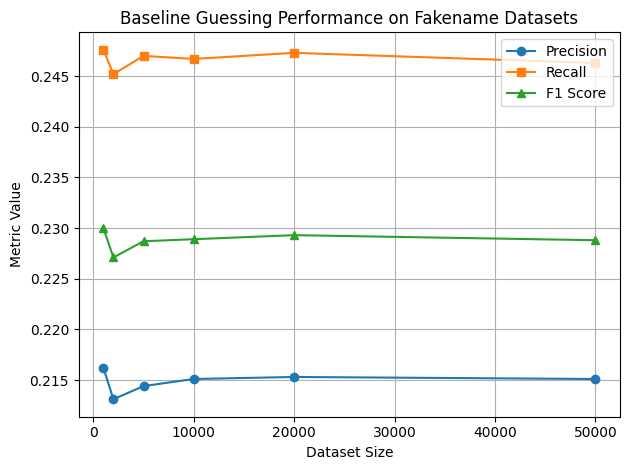
\includegraphics[width=0.7\textwidth]{img/fakename_analysis.png}
    \caption{Evaluation of the baseline performance on the \texttt{fakename} dataset: For each dataset size, the prediction quality of the 20 most frequent 2-grams is shown in terms of \textbf{precision}, \textbf{recall}, and \textbf{F1-score}. The average entry length is 21 characters.}
    \label{fig:baseline_metrics}
\end{figure}

For the \texttt{euro\_person} dataset, the baseline strategy for evaluating the effectiveness of the \ac{dea} follows the same procedure as for the \texttt{fakename} dataset.
Based on the analysis of this dataset, the average length of a full entry, comprising forename, surname, and full date of birth, is approximately 20 characters.
Assuming the use of 2-grams with overlapping character windows, this corresponds to around 19 distinct 2-grams per entry.
As a baseline, the top 19 most frequent 2-grams are selected and uniformly predicted for each record, independent of the individual characteristics of the entries.

The resulting performance metrics for this baseline prediction indicate a precision of 0.2197, a recall of 0.2446, and an F1-score of 0.2306.
These values provide an reference point for evaluating the added value of the \ac{dea} pipeline, as they quantify the effectiveness of a purely frequency driven reconstruction approach.

For the \texttt{titanic\_full} dataset, the average length of a full entry (consisting of given name and surname) is approximately 26 characters, indicating relatively high complexity due to longer names.
Therefore the top 25 most frequent 2-grams are selected as the baseline for reconstruction.
The baseline reconstruction approach achieved a precision of 0.2468, a recall of 0.3770, and an F1 score of 0.2896.
These modest performance values reflect the structural challenges posed by the dataset, including the presence of honorifics, compound names, and non-standard formatting.
The results suggest that even a naïve guessing strategy can establish a meaningful lower bound for evaluating the performance improvements of learning-based approaches such as the \ac{dea}.

Notably, for the \texttt{titanic\_full} dataset, the overlap ratio used in the experiments was adjusted to the set \{0.2, 0.4, 0.6, 0.7, 0.8, 0.9\}.
This adaptation was necessary because the dataset is relatively small, and the \ac{gma} fails to identify any individuals at lower overlap values.
Meaningful results only begin to emerge at an overlap of 0.7 or higher.

Notably, the similarity of the baseline metrics to those obtained on the \texttt{fakename} and \texttt{euro\_person} dataset highlights the generality of the method across synthetic and semi-realistic datasets, further justifying its inclusion as a comparative benchmark.

\section{Analysis}  \label{sec:analysis}

In this section the results of the \ac{dea} experiments are presented and analyzed.
The analysis is structured into several subsections, each focusing on a specific aspect of the \ac{dea} performance.
As described in Section~\ref{sec:experiments}, the experiments were conducted across multiple datasets, encoding schemes, overlaps and drop from strategies.
Therefore, several of these configuration settings will be fixed to analyze the impact of the remaining parameters on the \ac{dea} performance.

One important aspect especially for smaller datasets and overlap sizes is, that it could occur that the \ac{gma} does not identify any individuals, i.e., the re-identification set is empty.
In this case, the \ac{dea} is not able to reconstruct any plaintext information.
This is the case because if there are no re-identified individuals in place, there is no training data for the \ac{dea} available.
Therefore the results of these experiments are not reported and the corresponding data points are excluded from the analysis and plots.

The \ac{gma} could also fail during the attack by not being able to converge to a stable solution.
In this case, the \ac{dea} is not able to reconstruct any plaintext information as well.
Therefore the results of these experiments are not reported and the corresponding data points are excluded from the analysis and plots.

In total, 160 experiments were conducted to evaluate the attack's effectiveness under varying conditions, including different overlap levels and drop strategies.
On average, the \ac{dea} achieved a re-identification rate of 2.46\% and an F1-score of 0.621, with peak values reaching up to 22.68\% and 0.990, respectively.
Among the encoding schemes, \ac{tsh} exhibited the highest vulnerability with an average re-identification rate of 3.26\% and the best structural learnability (F1 = 0.682).
In contrast, \ac{tmh} yielded the lowest average re-identification rate (1.54\%), indicating greater resilience.
The following sections analyze these results in detail, focusing on how encoding choices, dataset characteristics, and attack configurations influence the \ac{dea}'s success.


\subsection{\ac{tmh}}

The following subsection focuses on the results obtained using the \ac{tmh} encoding scheme.
In this analysis, each dataset is evaluated under varying settings.
To ensure consistency, the dataset and encoding scheme are fixed, while the evaluation focuses on the impact of different overlap sizes and drop-from strategies.

\paragraph{Titanic Full}

On the \textit{Titanic Full} dataset, the \ac{dea} achieves stable and moderate performance using \ac{tmh} encoding.
The prediction quality improves consistently with increasing overlap between the auxiliary and target datasets (see Figure~\ref{fig:tabminhash_titanic} in Appendix~\ref{sec:tabminhash_results}).

For the \texttt{DropFrom = Eve} scenario, the F1-score decreases from 0.74 at overlap 0.7 to 0.17 at overlap 0.8, before recovering to 0.73 at overlap 0.9.
This dip at 0.8 is reflected in both recall and precision, suggesting a less effective hyperparameter configuration or reduced data utility at that particular overlap.
Precision is generally high across all overlaps, peaking at 0.96.

In the \texttt{DropFrom = Both} setting, the \ac{dea} maintains stable growth in both recall and F1-score.
Precision remains above 0.78 at all overlaps and reaches 0.96 at overlap 0.8.
At 0.9, the F1-score peaks at 0.72, confirming that even with this drop-from strategy, the \ac{dea} can learn meaningful patterns in \ac{tmh} encoded data.

Despite good predictive performance, no re-identification is achieved under any overlap or matching strategy.
Both fuzzy and greedy matching yield a re-identification rate of zero, underscoring the difficulty of exact record recovery on this small and heterogeneous dataset.

The comparison between F1-scores achieved during hyperparameter optimization (x-axis) and final trained F1-scores (y-axis) shows that the optimization procedure typically overestimates performance, with final trained scores being lower than those found during tuning, particularly at high-performing overlaps.
Nonetheless, the overall trend aligns well, indicating that hyperparameter optimization effectively identifies promising configurations.

In summary, the \ac{dea} demonstrates good structural learning on \ac{tmh} encoded Titanic data, particularly at higher overlaps, but fails to produce successful record re-identifications in this configuration.


\paragraph{Fakename 1k}

On the \textit{fakename 1k} dataset, the \ac{dea} demonstrates moderate predictive performance when using \ac{tmh} encoding (see Figure~\ref{fig:tabminhash_fakename1k} in Appendix~\ref{sec:tabminhash_results}).
The model's ability to recover n-gram patterns improves with increasing overlap, particularly in the \texttt{DropFrom = Eve} setting.

Under \texttt{DropFrom = Eve}, F1-scores increase from 0.18 at 0.4 overlap to 0.58 at 0.8 overlap.
This trend is mainly driven by improved recall, which rises from 0.10 to 0.43, while precision remains consistently high above 0.92.
This indicates that the \ac{dea} makes accurate predictions on a small but increasing portion of the encoded data as more re-identified data becomes available.

The \texttt{DropFrom = Both} configuration shows limited performance.
Although the F1-score improves from 0.00 to 0.22 between overlaps 0.4 and 0.8, recall stays low (below 0.14), and precision only surpasses 0.85 at the highest overlap.
This suggests that the model struggles to generalize well under this drop-from strategy.

Despite some structural learning success, the re-identification rate remains at zero across all overlap values and both drop-from strategies.
Neither greedy nor fuzzy matching yields any valid mappings to original records.

The comparison between F1-scores achieved during hyperparameter optimization and final trained F1-scores shows a generally accurate trend, with the optimization procedure typically overestimating performance (higher scores during tuning than final training), particularly in high-performing runs.
This suggests that the chosen Dice score remains a reliable metric during tuning despite the overestimation.

Overall, the \ac{dea} on \ac{tmh} encoded \textit{fakename 1k} data benefits from higher overlap and the \texttt{DropFrom = Eve} strategy but remains ineffective for precise record-level re-identification.


\paragraph{Fakename 2k}

On the \textit{fakename 2k} dataset, the \ac{dea} shows a clear improvement in predictive performance with increasing overlap when using \ac{tmh} encoding (see Figure~\ref{fig:tabminhash_fakename2k} in Appendix~\ref{sec:tabminhash_results}).
This trend is especially evident under the \texttt{DropFrom = Eve} configuration.

In the Eve setting, the F1-score increases from 0.10 at 0.4 overlap to 0.57 at 0.6, reaching 0.73 at 0.8.
This is driven by steady improvements in recall (from 0.06 to 0.62), while precision remains consistently high (above 0.90 at both 0.4 and 0.8).
These results suggest that the \ac{dea} learns meaningful structural patterns when sufficient re-identified training data is available.

The \texttt{DropFrom = Both} scenario shows much weaker performance.
The F1-score only reaches 0.16 at overlap 0.8, with recall staying below 0.11 and precision peaking at just 0.35.
This indicates that the \texttt{DropFrom = Both} strategy significantly limits the learning signal on smaller datasets, reducing the \ac{dea}'s effectiveness.

Re-identification remains unsuccessful across all configurations and overlaps.
Neither fuzzy nor greedy matching methods yield any valid re-identifications, which reflects the difficulty of achieving exact plaintext recovery in low-coverage scenarios.

Hyperparameter optimization typically overestimates the final trained F1-scores for all configurations (higher scores during tuning than final training), though the trend is consistent and particularly close for higher-overlap Eve settings.
This suggests the tuning metric (Dice score) remains informative for model selection despite the overestimation.

In summary, \ac{tmh} encoding on the \textit{fakename 2k} dataset enables effective n-gram prediction under the \texttt{DropFrom = Eve} strategy, while re-identification remains out of reach under all tested conditions.


\paragraph{Fakename 5k}

For the \textit{fakename 5k} dataset, the \ac{dea} achieves strong performance in reconstructing structural patterns when \ac{tmh} is used (see Figure~\ref{fig:tabminhash_fakename5k} in Appendix~\ref{sec:tabminhash_results}).
Both \texttt{DropFrom = Eve} and \texttt{DropFrom = Both} settings show substantial improvements in predictive quality with increasing overlap.

In the \texttt{DropFrom = Eve} scenario, the F1-score rises from 0.14 at 0.2 overlap to a peak of 0.87 at 0.6.
This is supported by a corresponding increase in recall from 0.11 to 0.80, while precision exceeds 0.95 from 0.4 onward.
The \texttt{DropFrom = Both} configuration follows a similar trend, achieving an F1-score of 0.77 at 0.6 overlap, with precision of 0.98 and recall around 0.65.

Notably, this is the first setting in which the \ac{dea} yields non-zero re-identification rates.
In the \texttt{DropFrom = Eve} configuration, a re-identification rate of 1.2\% is observed at 0.6 overlap, with contributions from both fuzzy and greedy matching.
The \texttt{DropFrom = Both} setting shows a smaller but non-negligible rate of 0.07\% at the same overlap.
These results mark the transition from structural to record-level leakage under favorable training conditions.

Hyperparameter optimization correlates well with final model performance.
While the F1-scores achieved during hyperparameter optimization typically overestimate the final trained F1-scores (higher during tuning than final training), the trends remain aligned and the top-performing models match closely with the best configurations found during tuning.

Overall, this setting demonstrates that the \ac{dea} can become effective at re-identification as dataset size and training overlap increase.
\ac{tmh} encoded \ac{pii} becomes vulnerable to both structural inference and, under certain conditions, full record re-identification.


\paragraph{Fakename 10k}

The \ac{dea} achieves high performance on the \textit{fakename 10k} dataset with \ac{tmh} encoding (see Figure~\ref{fig:tabminhash_fakename10k} in Appendix~\ref{sec:tabminhash_results}).
Both predictive quality and re-identification effectiveness increase significantly with overlap, particularly under the \texttt{DropFrom = Eve} scenario.

In the Eve setting, the F1-score improves from 0.51 at 0.2 overlap to 0.93 at 0.6 and 0.92 at 0.8.
Precision remains consistently above 0.96, and recall exceeds 0.9 at the two highest overlaps.
The model clearly benefits from access to a larger fraction of re-identified training data, leading to near-perfect structural reconstruction.

The \texttt{DropFrom = Both} configuration follows a similar trend but with slightly lower performance at small overlaps.
At 0.8 overlap, it reaches an F1-score of 0.91, with precision of 0.98 and recall of 0.86.
Compared to smaller datasets, performance differences between the two dropout strategies become marginal at high overlaps.

For the first time, substantial re-identification rates are observed.
Under \texttt{DropFrom = Eve}, the combined re-identification rate reaches 5.45\% at 0.6 overlap and remains above 5\% at 0.8.
The \texttt{DropFrom = Both} configuration achieves a lower peak of 2.97\% at 0.8.
Both fuzzy and greedy methods contribute to these results, with fuzzy matching consistently recovering more records.

These findings are mirrored in the aggregate relationship between F1-score and re-identification rate, which shows a clear positive correlation. This confirms that structural accuracy translates to successful record-level attacks in larger datasets.

The F1-scores achieved during hyperparameter optimization closely track the final trained values, particularly for the high-performing configurations, though typically with slight overestimation (higher scores during tuning than final training).
The Dice score used for tuning appears well-calibrated even in high-dimensional settings.

Overall, the \ac{dea} is highly effective on \ac{tmh} encoded data when training coverage is sufficient and dataset size enables generalization.
The combination of high recall and precision leads to significant re-identification risk at overlap levels of 0.6 and above.


\paragraph{Fakename 20k}

The \ac{dea} reaches its highest level of effectiveness on the \textit{fakename 20k} dataset when using \ac{tmh} encoding (see Figure~\ref{fig:tabminhash_fakename20k} in Appendix~\ref{sec:tabminhash_results}).
Both structural reconstruction and re-identification performance scale with dataset size and overlap, confirming the vulnerability of \ac{tmh} encoded data under \ac{dea}s.

In the \texttt{DropFrom = Eve} configuration, F1-scores increase from 0.51 at 0.2 overlap to 0.96 at 0.8.
Precision and recall both exceed 0.95 at the highest overlap, indicating that the model is able to reconstruct the n-gram distribution with high fidelity.
The \texttt{DropFrom = Both} setting follows a similar trajectory, with the F1-score reaching 0.95 at 0.8 and precision nearly identical to the Eve scenario.

The re-identification rates increase sharply with overlap.
Under \texttt{DropFrom = Eve}, the combined re-identification rate reaches 13.47\% at 0.8, with greedy and fuzzy matching each contributing a substantial portion.
Even in the more conservative \texttt{DropFrom = Both} setting, the rate surpasses 10\% at the highest overlap, confirming that re-identification is possible even without access to a clean subset.

The correlation between F1-score and re-identification rate is stronger than in previous datasets, with a visibly steep upward trend.
This suggests that small improvements in structural accuracy have increasingly large effects on re-identification success in large-scale datasets.

The hyperparameter optimization results are tightly aligned with final model performance, particularly for configurations with F1-scores above 0.9, though typically with slight overestimation (higher scores during tuning than final training).
The Dice score remains a reliable proxy for selecting high-performing models in high-dimensional learning scenarios.

In summary, the \textit{fakename 20k} experiments demonstrate the full potential of the \ac{dea}.
With high overlap and sufficient data, \ac{tmh} encoding fails to protect against meaningful reconstruction and record-level compromise.


\paragraph{Europerson}

The \textit{euro person} dataset further confirms the vulnerability of \ac{tmh} encodings under \ac{dea}s (see Figure~\ref{fig:tabminhash_euro} in Appendix~\ref{sec:tabminhash_results}).
Despite variations in overlap, the \ac{dea} consistently achieves high predictive performance and exhibits meaningful re-identification capability.

Across all overlap values, the model maintains high precision (above 0.92), with only moderate variability in recall.
In the \texttt{DropFrom = Both} setting, F1-scores exceed 0.87 at all overlaps and peak at 0.94 for overlap 0.4.
The \texttt{DropFrom = Eve} configuration shows more fluctuation, with F1-scores ranging from 0.50 to 0.92, likely due to reduced training set size at lower overlaps.

Re-identification rates vary substantially across overlaps.
In the \texttt{DropFrom = Both} setting, a peak re-identification rate of 6.85\% is observed at overlap 0.6.
Notably, this rate drops to near zero at 0.8, despite similar predictive metrics, indicating the effect of reduced unique reconstruction under high training similarity.
The \texttt{DropFrom = Eve} setting shows similar behavior with a maximum re-identification rate of 6.12\% at 0.6 overlap, largely driven by greedy matches.

The aggregate F1-to-re-identification relationship exhibits a clear positive trend, reinforcing that high structural accuracy translates into privacy loss at the record level.
This is further supported by the distribution of fuzzy and greedy re-identifications, with both contributing significantly at intermediate overlaps.

Hyperparameter optimization yields slightly optimistic F1-scores in some runs (higher scores during tuning than final training), but the trained values remain closely aligned overall.
The Dice score again proves to be a stable tuning criterion.

Overall, the \textit{euro person} dataset reveals that even realistic data encoded via \ac{tmh} is susceptible to reconstruction and re-identification.
The \ac{dea} performs reliably across settings, with overlap 0.6 appearing to maximize re-identification success.


\paragraph{Summary Across Datasets and Overlap Levels}

Figure~\ref{fig:tabminhash_overlap} in Appendix~\ref{sec:tabminhash_results} illustrates the relationship between overlap and both re-identification rate (left) and F1-score (right), averaged over drop strategies for each dataset.
The results highlight how both structural and record-level vulnerabilities evolve with dataset size and training coverage.

Larger datasets such as \textit{fakename 20k}, \textit{fakename 10k}, and \textit{euro person} exhibit clear monotonic trends.
As the overlap increases, both F1-scores and re-identification rates improve.
For \textit{fakename 20k}, the re-identification rate peaks at nearly 12\% for 0.8 overlap.
Similarly, \textit{euro person} reaches its highest F1-score at 0.6 overlap, accompanied by its highest re-identification performance, indicating that structural accuracy enables effective exploitation.

Smaller datasets such as \textit{fakename 1k}, \textit{2k}, and \textit{titanic full} show limited gains in re-identification, regardless of overlap.
Their F1-scores increase with overlap, but remain insufficient to enable consistent reconstruction.
Notably, \textit{fakename 5k} serves as a transition point: at 0.6 overlap, it achieves a modest re-identification rate and solid F1-score, but both metrics drop again at 0.8 overlap.

Across datasets, the plots reveal that higher overlap generally yields better F1-scores.
However, effective re-identification is highly dependent on dataset size and complexity.
The correlation between these two metrics is dataset-specific and non-linear, particularly at high F1 values where small increases may lead to steep jumps in re-identification.

These findings reinforce the conclusion that \ac{tmh} encodings do not provide sufficient protection in high-overlap, large-scale scenarios.
While the \ac{dea} may remain ineffective on small or disjoint datasets, it becomes increasingly potent as structural learning converges, ultimately compromising encoded identifiers.

\paragraph{Architecture}

Figure~\ref{fig:tabminhash_architecture} in Appendix~\ref{sec:tabminhash_results} presents a distributional analysis of the neural network architectures selected during hyperparameter optimization across all \ac{tmh} experiments.
The results provide insight into which architectural choices consistently yield strong performance in structural reconstruction and re-identification tasks.

The majority of optimized models employ a shallow architecture with a single hidden layer.
More complex configurations with two or three layers are rare, suggesting that the \ac{dea} can learn effective representations without requiring deep hierarchical abstraction.
This is consistent with the relatively structured nature of the prediction task and the compactness of \ac{tmh} encoded records.

In terms of hidden size, larger configurations are clearly favored.
The most frequent choice is a hidden dimension of 2048, followed by 1024.
Smaller sizes below 512 occur infrequently, indicating that wide layers contribute significantly to capturing the necessary n-gram co-occurrence patterns for decoding.

Dropout rates are broadly distributed, with a mean around 0.24.
This suggests that regularization is helpful, but not critical; overfitting appears to be limited even with lower dropout.
The threshold histogram indicates that models typically settle around a value of 0.44 for binary classification, though a wide range is explored, reflecting dataset-specific optimality.

Activation functions are led by \texttt{elu} and \texttt{selu}, both of which support smooth non-linear transitions and internal normalization.
Simpler functions like \texttt{relu} and \texttt{gelu} are used less frequently.
This preference for normalized activations may reflect the benefits of stability during training on small gradients.

Among optimizers, \texttt{AdamW} is most commonly selected, followed by \texttt{Adam} and \texttt{\texttt{RMSprop}}.
This aligns with the need for stable adaptive learning rates and effective weight decay.
Learning rate schedulers are also diverse, with \texttt{ReduceLROnPlateau} and \texttt{CyclicLR} being the most frequent.
The inclusion of schedulers reflects their utility in adjusting learning dynamics over the short training windows.

Batch sizes of 8 and 16 dominate, likely due to the small to medium dataset sizes and the use of non-GPU resource constraints during experimentation.
Finally, the number of training epochs converges to 20 in nearly all cases, the maximum allowed during tuning, suggesting that performance continues to improve up to the epoch limit.

In summary, the optimal architecture for \ac{tmh} encoded \ac{dea} models is characterized by a shallow but wide feedforward network, mild regularization, normalized activations, and adaptive optimizers with scheduler support.
These configurations are robust across datasets and contribute significantly to the attack's effectiveness.

\subsection{\ac{tsh}}

The following subsection focuses on the results obtained using the \ac{tsh} encoding scheme.
In this analysis, each dataset is evaluated under varying settings.
To ensure consistency, the dataset and encoding scheme are fixed, while the evaluation focuses on the impact of different overlap sizes and drop-from strategies.

\paragraph{Titanic Full}

On the \textit{Titanic Full} dataset, the \ac{dea} performs reliably when using \ac{tsh} encoding, achieving stable precision and recall across overlap values (see Figure~\ref{fig:twostep_titanic} in Appendix~\ref{sec:twostep_results}).
F1-scores range from 0.34 to 0.83, depending on the drop strategy and overlap.

In the \texttt{DropFrom = Eve} setting, the model consistently achieves high precision (above 0.95) across all tested overlaps.
Recall improves with overlap, rising from 0.56 at 0.7 to 0.74 at 0.9.
The resulting F1-score increases accordingly, reaching a maximum of 0.83 at 0.9 overlap, indicating robust learning from partially re-identified data even in small datasets.

The \texttt{DropFrom = Both} configuration shows more variability.
At 0.7 overlap, the F1-score remains low at 0.34, reflecting low precision (0.26) despite moderate recall (0.55).
However, at 0.8 overlap, both precision and recall improve, yielding an F1-score of 0.72.
This suggests that the \texttt{DropFrom = Both} strategy can be mitigated as overlap increases, but model reliability depends strongly on sample size.

No re-identifications are observed at any overlap level for either drop-from strategy.
Both fuzzy and greedy matching yield zero hits, highlighting that accurate structural predictions do not necessarily lead to successful record reconstruction in small datasets like \textit{Titanic Full}.

The comparison of trained and optimized F1-scores shows good alignment, with optimization results slightly underestimating final model performance.
The Dice score remains a useful surrogate during tuning, especially for mid-range overlaps.

In summary, \ac{tsh} provides solid predictive performance on the \textit{Titanic Full} dataset, particularly when Eve's overlap is high.
Nonetheless, the attack remains structurally bounded, and record-level re-identification is not achieved.


\paragraph{Fakename 1k}

On the \textit{fakename 1k} dataset, the \ac{dea} shows measurable improvements in structural prediction performance as the overlap increases, though it fails to achieve any successful re-identifications (see Figure~\ref{fig:twostep_fakename1k} in Appendix~\ref{sec:twostep_results}).

In the \texttt{DropFrom = Eve} setting, F1-scores rise sharply with overlap, starting from 0.11 at 0.4 to 0.74 at 0.8.
This trend is driven by improvements in both recall (from 0.06 to 0.62) and precision (from 0.52 to 0.95).
The results suggest that the \ac{dea} is able to learn useful representations even with a small dataset, provided sufficient re-identified training data is available.

The \texttt{DropFrom = Both} configuration performs worse, particularly at lower overlaps.
At 0.6 overlap, F1-score remains low (0.07), but rises to 0.66 at 0.8, supported by high precision (0.95) and moderate recall (0.52).
This indicates that the \texttt{DropFrom = Both} strategy is more detrimental at small scale, though sufficient overlap mitigates this effect.

Despite achieving F1-scores over 0.7 in some configurations, re-identification remains at 0\% for all tested overlaps and matching strategies.
This underlines the fact that a strong n-gram prediction model does not necessarily translate into record-level success when the dataset size is small.

The comparison between optimized and trained F1-scores is consistent, with only minor deviations.
The hyperparameter tuning process based on Dice/F1 remains reliable even in data-scarce settings.

Overall, \ac{tsh} yields competitive structural predictions on small datasets like \textit{fakename 1k}, particularly when the training overlap is high.
However, the \ac{dea} does not succeed in reconstructing any individual records in this configuration.



\paragraph{Fakename 2k}

The \textit{fakename 2k} dataset reveals a clear improvement in \ac{dea} performance with increasing overlap when \ac{tsh} encoding is used (see Figure~\ref{fig:twostep_fakename2k} in Appendix~\ref{sec:twostep_results}).
While low-overlap configurations perform poorly, both structural prediction and re-identification become feasible at higher overlaps.

In the \texttt{DropFrom = Eve} setting, the F1-score increases from 0.11 at 0.2 to 0.76 at 0.6, and further to 0.83 at 0.8.
Precision remains high throughout (above 0.79), while recall improves substantially with overlap, reaching 0.76 and 0.76 at 0.6 and 0.8, respectively.
These results indicate that once a sufficient number of re-identified records are available, the \ac{dea} can learn and generalize the underlying encoding structure effectively.

The \texttt{DropFrom = Both} configuration follows a similar trend but lags slightly.
At 0.4 overlap, performance remains negligible (F1 = 0.11), but at 0.8 it rises to 0.83, with both precision (0.97) and recall (0.74) being strong.
This confirms that the \texttt{DropFrom = Both} strategy can be overcome given sufficient overlap.

Unlike on the 1k dataset, the \ac{dea} successfully re-identifies individual records at higher overlaps. Under \texttt{DropFrom = Eve}, a small re-identification rate of 0.1\% is achieved at 0.6.
In the \texttt{DropFrom = Both} setting, this increases to 0.3\% at 0.8.
Although the rates are modest, they demonstrate that re-identification becomes possible as structural accuracy increases.

The trend between F1-score and re-identification rate is consistent, with successful re-identifications only occurring beyond F1 = 0.75.
This reflects a threshold-like behavior in the attack's effectiveness.

Hyperparameter tuning correlates well with trained outcomes.
In particular, the optimized Dice scores closely match final F1-scores for the best configurations, validating the use of Dice as a selection criterion.

In summary, the \textit{fakename 2k} dataset shows that \ac{tsh} encoding provides limited protection once the overlap exceeds 0.6.
The \ac{dea} can achieve strong predictions and initial re-identifications even in modestly sized datasets.


\paragraph{Fakename 5k}

The \textit{fakename 5k} dataset marks the transition point where the \ac{dea} begins to yield meaningful re-identification rates under \ac{tsh} encoding (see Figure~\ref{fig:twostep_fakename5k} in Appendix~\ref{sec:twostep_results}).
Both precision and recall improve steadily with increasing overlap, and re-identification becomes feasible.

In the \texttt{DropFrom = Eve} setting, the model achieves an F1-score of 0.10 at 0.2 overlap, but quickly improves to 0.89 at 0.6, with near-perfect precision (0.99) and strong recall (0.82).
Interestingly, performance slightly drops at 0.8, suggesting that the increased overlap does not always translate to higher generalization capacity under this drop strategy.

The \texttt{DropFrom = Both} configuration follows a smoother trajectory.
F1-score increases from 0.22 at 0.2 overlap to 0.76 at 0.4, 0.89 at 0.6, and peaks at 0.94 at 0.8.
These results are underpinned by consistently high precision and rising recall, indicating the model's ability to capture \ac{tmh} encoded structure even under the \texttt{DropFrom = Both} strategy.

The first substantial re-identification rates are observed in this dataset.
Under \texttt{DropFrom = Eve}, the combined rate reaches 2.1\% at 0.6 but drops again at 0.8.
In contrast, \texttt{DropFrom = Both} shows increasing re-identification, reaching 5.52\% at 0.8.
This inverse pattern suggests that different dropout strategies interact differently with the learned representations, particularly when Eve's dataset becomes large and less diverse.

The re-identification curve as a function of F1-score shows the expected upward trend, confirming that strong structural prediction is a prerequisite for record-level re-identification.

Hyperparameter optimization is effective across all configurations.
F1-scores achieved during hyperparameter optimization are typically slightly optimistic (higher during tuning than final training) but closely follow the trend of the final trained models.

Overall, the \textit{fakename 5k} dataset demonstrates that \ac{dea} success under \ac{tsh} encoding is strongly dependent on overlap and dataset size.
Once a critical threshold is reached, even structurally obfuscated data becomes vulnerable to reconstruction.



\paragraph{Fakename 10k}

The \ac{dea} achieves consistently high structural prediction performance on the \textit{fakename 10k} dataset when using \ac{tsh} encoding (see Figure~\ref{fig:twostep_fakename10k} in Appendix~\ref{sec:twostep_results}).
Re-identification becomes substantial, particularly in the \texttt{DropFrom = Eve} configuration at intermediate overlaps.

In the Eve setting, F1-scores are strong across all overlaps: 0.87 at 0.2, rising to 0.94 at 0.6, before slightly decreasing to 0.75 at 0.8.
These fluctuations are primarily driven by changes in recall, which peaks at 0.90 but drops sharply at 0.8, despite stable precision above 0.96 throughout.
This indicates that excessive overlap may not always improve performance due to overfitting or reduced variance in the training set.

The \texttt{DropFrom = Both} configuration shows more stability at high overlaps.
F1-scores increase from 0.76 at 0.2 to 0.91 at 0.4, and finally 0.94 at 0.8.
At 0.6, however, the model fails to generalize, with recall collapsing to 0.05 and F1 dropping to 0.10.
This suggests a sensitivity to training set composition at this overlap.

Re-identification rates are highest for Eve at 0.6 overlap (10.9\%), coinciding with its peak in F1-score.
The \texttt{DropFrom = Both} setup reaches a maximum re-identification rate of 5.6\% at 0.8.
Fuzzy and greedy matching contribute similarly to the results, with combined predictions amplifying the attack's effectiveness.

The re-identification rate shows a non-linear but positively correlated relationship with F1-score.
The strongest privacy breaches occur in the range F1 > 0.9, highlighting the tipping point at which structural reconstruction translates into record-level compromise.

Hyperparameter optimization continues to perform reliably, with trained F1-scores closely tracking the optimal Dice values across overlaps.

In summary, the fakename 10k dataset confirms that \ac{dea} success under \ac{tsh} encoding scales with dataset size and overlap.
However, unexpected performance drops can occur under certain dropout conditions, emphasizing the need for robust model selection.


\paragraph{Fakename 20k}

The \textit{fakename 20k} dataset confirms the scalability and effectiveness of the \ac{dea} when applied to large, \ac{tsh} encoded datasets (see Figure~\ref{fig:twostep_fakename20k} in Appendix~\ref{sec:twostep_results}).

In the \texttt{DropFrom = Eve} configuration, the \ac{dea} achieves F1-scores of 0.94 and 0.97 at overlaps 0.2 and 0.4, respectively.
Both precision and recall are near 1.0, indicating highly reliable reconstruction of the encoded representations.
In the \texttt{DropFrom = Both} case, the model achieves an F1-score of 0.92 at 0.8 overlap with precision of 0.99 and recall of 0.86, again showing strong generalization under symmetric dropout.

Re-identification rates are substantial.
Under \texttt{DropFrom = Eve}, the rate increases from 5.73\% at 0.2 overlap to 13.20\% at 0.4.
The combined matching strategy benefits from contributions by both fuzzy and greedy methods, peaking at over 13\%.

In the \texttt{DropFrom = Both} setting, the re-identification rate reaches 2.49\% at 0.8 overlap.
While lower than in the Eve case, this still represents a notable privacy breach, particularly under conditions where no cleartext subset is available to the attacker.

The positive linear trend between F1-score and re-identification rate is especially clear in this dataset, with a nearly perfect fit across configurations.
This reinforces the conclusion that once structural accuracy exceeds 0.9, re-identification becomes a likely outcome.

Hyperparameter optimization results align tightly with final F1-scores, though typically with slight overestimation during the optimization phase (higher scores during tuning than final training).
The Dice score again proves to be an effective and well-calibrated tuning metric for large-scale datasets.

In summary, the \textit{fakename 20k} experiments demonstrate high vulnerability of \ac{tsh} encoded databases under \ac{dea}s.
Even with minimal overlap, the \ac{dea} can achieve both high reconstruction fidelity and impactful re-identification, posing a serious threat to encoded privacy-preserving record linkage.


\paragraph{Europerson}

The \textit{euro\_person} dataset yields the highest observed re-identification rates under \ac{tsh} encoding.
Structural prediction performance is nearly perfect across all overlap values, and re-identification success exceeds 20\% at high overlap.

In the \texttt{DropFrom = Eve} configuration, the model achieves F1-scores above 0.98 for overlaps 0.6 and 0.8.
Precision and recall are both near 1.0, indicating that the model captures the encoded structure with high fidelity.
Even at 0.2 overlap, the F1-score remains strong at 0.93, supported by a recall of 0.90 and precision of 0.95.

The \texttt{DropFrom = Both} setting shows similar behavior.
The F1-score rises from 0.68 at 0.2 to 0.98 at 0.6 and 0.99 at 0.8.
This suggests that sufficient overlap renders the \ac{dea} robust even under this drop-from strategy.

Re-identification rates are particularly striking.
Under \texttt{DropFrom = Eve}, the combined matching method reaches 22.6\% at 0.6 overlap and remains stable at 22.3\% at 0.8.
The corresponding values in the \texttt{DropFrom = Both} setting are 17.8\% and 21.9\%, respectively.
These are the highest attack success rates recorded, highlighting the severe privacy risk associated with large, European-style datasets and well-optimized neural architectures.

The re-identification curve versus F1-score shows a near-linear relationship with a steep slope, underscoring the strong coupling between model accuracy and privacy leakage.

Hyperparameter optimization is effective.
The predicted F1-scores during tuning closely match the final trained values, and tuning time remains tractable even for large dataset sizes.

In summary, the \textit{euro\_person} dataset illustrates that the combination of \ac{tsh} encoding and realistic, high-quality input data is particularly vulnerable to \ac{dea}s.
The \ac{dea} can achieve both high prediction fidelity and extensive re-identification success, even with limited initial overlap.

\paragraph{Summary Across Datasets and Overlap Levels}

The summary plots in Figure~\ref{fig:twostep_overlap} in Appendix~\ref{sec:twostep_results} illustrate the overall relationship between overlap, structural prediction quality, and re-identification success across all evaluated datasets using \ac{tsh} encoding.

Across all datasets, F1-scores generally increase with overlap, reflecting improved structural learning by the neural model as more training data becomes available.
For small datasets like \textit{titanic full} and \textit{fakename 1k}, the \ac{dea} struggles until the overlap reaches 0.8.
In contrast, medium-sized datasets such as \textit{fakename 5k} and \textit{10k} show rapid improvement between 0.4 and 0.6.
Larger datasets (\textit{fakename 20k} and \textit{euro\_person}) achieve F1-scores above 0.9 even at lower overlaps (0.2 or 0.4), confirming their higher learnability.

Re-identification success remains low in small datasets, regardless of F1-score.
In \textit{fakename 1k}, \textit{2k}, and \textit{titanic full}, the \ac{dea} fails to re-identify any records.
The first meaningful re-identification rates emerge in \textit{fakename 5k}, with up to 5.5\% at high overlap.
In \textit{fakename 10k}, the rate peaks at 10.9\% but drops slightly at 0.8.
\textit{Fakename 20k} shows a more irregular pattern, with a maximum of 13.2\% at 0.4 but a slight decline thereafter.
The \textit{euro\_person} dataset is the most vulnerable, with re-identification rates exceeding 22\% at 0.6 and 0.8.

These results confirm a non-linear but consistent dependency between structural performance and re-identification capability.
Notably, some datasets exhibit diminishing returns at very high overlaps, potentially due to reduced variability or model overfitting.
Additionally, privacy leakage appears to depend not only on model performance (F1) but also on dataset characteristics such as name structure, token diversity, and size.

Overall, \ac{tsh} poses a clear privacy risk under \ac{dea}s.
While encoding obfuscates raw values, neural networks trained on auxiliary data can learn the structural mapping and enable re-identification—especially in realistic, large-scale datasets.

\paragraph{Architecture}

Figure~\ref{fig:twostep_architecture} in Appendix~\ref{sec:twostep_results} shows the distributions of the best-performing neural network configurations for models trained on \ac{tsh} encoded datasets.
Most models are relatively shallow: the majority use a single hidden layer, indicating that deeper networks are not necessary to capture the structure of the encoding.
At the same time, the preferred hidden size is large, with 2048 being the most frequent choice, suggesting that a wide representation is crucial for learning the mapping from encoded inputs to class labels.

In terms of activation functions, \texttt{gelu} and \texttt{selu} are most often selected, while traditional choices like \texttt{relu}, \texttt{tanh}, and \texttt{leaky\_relu} appear less frequently.
This preference points to the importance of smooth and differentiable non-linearities that preserve gradient flow, especially when working with hashed inputs.
Optimizer selection favors \texttt{RMSprop}, followed by Adam and AdamW.
\texttt{RMSprop}'s popularity may be due to its ability to handle sparse and noisy gradients effectively.
Learning rate schedulers are used in most cases, with \texttt{None} and \texttt{CyclicLR} dominating.
This reflects that both fixed and adaptive schedules can work well depending on dataset size and overlap.

Regularization is handled via dropout, with most selected values ranging between 0.15 and 0.35 (mean: 0.25), indicating a moderate level of regularization is helpful to avoid overfitting to the structure of the extended training data.
The decision threshold for classification tends to cluster around 0.39, which reflects the model's calibrated confidence when predicting links.
Most models train for around 15–20 epochs, with a noticeable concentration at the upper bound, suggesting that full training cycles are often required to reach convergence.
Small batch sizes, particularly 8 and 16, dominate, likely due to their regularizing effect and suitability for noisy structural input.

\subsection{\ac{bf}}

The following subsection focuses on the results obtained using the \ac{bf} encoding scheme.
In this analysis, each dataset is evaluated under varying settings.
To ensure consistency, the dataset and encoding scheme are fixed, while the evaluation focuses on the impact of different overlap sizes and drop-from strategies.

\paragraph{Titanic Full}

On the \textit{Titanic Full} dataset, the \ac{dea} demonstrates strong structural learning capabilities when using \ac{bf} encoding (see Figure~\ref{fig:bloomfilter_titanic} in Appendix~\ref{sec:bloomfilter_results}).

At overlap 0.9, the model reaches an F1-score of 0.83 under the \texttt{DropFrom = Eve} strategy, indicating that the structural mapping between encoded and raw data can be learned to a high degree.
When training on data dropped from both parties, the model performs slightly worse with an F1-score of 0.81.
While the precision is consistently high in both cases (above 0.95), recall increases significantly with higher overlap and is consistently better when training on Eve's removed data.

Despite strong structural performance, no successful re-identifications were made, regardless of overlap or re-identification strategy.
Both fuzzy and greedy matching yield zero hits, highlighting that accurate structural predictions do not necessarily lead to successful record reconstruction in small datasets like \textit{Titanic Full}.

The comparison of final trained F1-scores with those achieved during hyperparameter optimization shows good alignment, with optimization results typically overestimating final model performance (higher scores during tuning than final training).
The Dice score remains a useful surrogate during tuning, especially for high overlaps.

In summary, \ac{bf} provides solid predictive performance on the \textit{Titanic Full} dataset, particularly when Eve's overlap is high.
Nonetheless, the attack remains structurally bounded, and record-level re-identification is not achieved.

\paragraph{Fakename 1k}

On the \textit{fakename 1k} dataset, the \ac{dea} shows moderate performance when using \ac{bf} encoding (see Figure~\ref{fig:bloomfilter_fakename1k} in Appendix~\ref{sec:bloomfilter_results}).
Performance varies notably depending on the drop strategy.

Under the \texttt{DropFrom = Eve} setting, the model achieves a peak F1-score of 0.67 at overlap 0.8.
Precision reaches over 0.9, while recall follows a similar trend, confirming that overlap and drop strategy significantly influence learnability.

The \texttt{DropFrom = Both} configuration shows consistently lower performance, with F1-scores never exceeding 0.20.
Precision remains low for this strategy, indicating that the model struggles to generalize well under this drop-from strategy.

Despite the difference in structural performance, no re-identifications are made at any overlap or with any matching method.
As before, the attack manages to recover structural patterns when training data is suitable, but \ac{bf}s at this scale appear to prevent any meaningful semantic reconstruction.

The comparison between F1-scores achieved during hyperparameter optimization and final trained F1-scores shows generally accurate trends, with the optimization procedure typically overestimating performance (higher scores during tuning than final training), particularly in high-performing runs.

Overall, \ac{bf} yields competitive structural predictions on small datasets like \textit{fakename 1k}, particularly when the training overlap is high.
However, the \ac{dea} does not succeed in reconstructing any individual records in this configuration.

\paragraph{Fakename 2k}

For the \textit{fakename 2k} dataset, the \ac{dea} shows clear improvement in predictive performance with increasing overlap when \ac{bf} encoding is used (see Figure~\ref{fig:bloomfilter_fakename2k} in Appendix~\ref{sec:bloomfilter_results}).

Under the \texttt{DropFrom = Eve} setting, the attack reaches an F1-score of 0.86 at overlap 0.8.
This is supported by both precision and recall exceeding 0.8, indicating robust learning from partially re-identified data.

The \texttt{DropFrom = Both} configuration shows weaker performance, yielding an F1-score of 0.72 at the same overlap.
This discrepancy mirrors the gap in recall and precision between the two conditions, with recall remaining below 0.7 for the Both strategy.

Unlike previous datasets, \ac{bf} encoding begins to show measurable vulnerability.
The re-identification rate reaches 1.5\% in the best case (overlap 0.8, \texttt{DropFrom = Eve}), with most successful re-identifications resulting from the fuzzy matching strategy.+

The comparison between F1-score and re-identification rate shows a clear positive correlation, confirming that structural accuracy translates to successful record-level attacks.

Hyperparameter optimization correlates well with final model performance, with F1-scores achieved during optimization typically overestimating the final trained values (higher scores during tuning than final training).

In summary, the \textit{fakename 2k} dataset shows that \ac{bf} encoding provides limited protection once the overlap exceeds 0.8.
The \ac{dea} can achieve strong predictions and initial re-identifications even in modestly sized datasets.

\paragraph{Fakename 5k}

The \textit{fakename 5k} dataset exhibits a noticeable rise in vulnerability under \ac{bf} encoding (see Figure~\ref{fig:bloomfilter_fakename5k} in Appendix~\ref{sec:bloomfilter_results}).

At overlap 0.6, the model trained on \texttt{DropFrom = Eve}  achieves an F1-score of 0.93, clearly surpassing the performance of the model trained with the \texttt{DropFrom = Both} strategy (F1 = 0.90).
For overlap 0.8, the scores diverge more strongly: the F1-score drops to 0.49 for \texttt{DropFrom = Eve}, while it remains high at 0.87 for \texttt{DropFrom = Both}.
This inversion suggests a shift in learning dynamics where a larger overlap allows the model trained on \texttt{DropFrom = Both} to generalize better, possibly due to higher variance in the training set.

The re-identification rate peaks at overlap 0.6, with 5.1\% when trained on \texttt{DropFrom = Eve} and 1.6\% for \texttt{DropFrom = Both}.
In both cases, the combined matching method yields the majority of successful links, while fuzzy and greedy individually contribute smaller fractions.

Compared to \textit{fakename 2k}, the attacker gains more leverage here.
While the F1-score improves only slightly, the re-identification rate scales more than threefold, indicating that higher dataset contributes to exploitability.

The re-identification curve as a function of F1-score shows the expected upward trend, confirming that strong structural prediction is a prerequisite for record-level re-identification.

Hyperparameter optimization is effective across all configurations, with F1-scores achieved during optimization typically overestimating the final trained values (higher scores during tuning than final training) but closely following the trend of the final trained models.

Overall, the \textit{fakename 5k} dataset demonstrates that \ac{dea} success under \ac{bf} encoding is strongly dependent on overlap and dataset size.
Once a critical threshold is reached, even structurally obfuscated data becomes vulnerable to reconstruction.

\paragraph{Fakename 10k}

The results on \textit{fakename 10k} mark a transition into a regime where the dataset size and model capacity jointly enable highly effective re-identification under \ac{bf} encoding (see Figure~\ref{fig:bloomfilter_fakename10k} in Appendix~\ref{sec:bloomfilter_results}).

The F1-score reaches a peak of 0.95 for \texttt{DropFrom = Eve} and 0.94 for \texttt{DropFrom = Both} at overlap 0.6.
For both drop-from strategies, this overlap corresponds to the best-performing configuration.
At overlap 0.8, both models maintain high performance, although \texttt{DropFrom = Both} starts to degrade more steeply (F1 = 0.81 vs. 0.88 for Eve).

Re-identification is most successful at overlap 0.6, with rates of 11.1\% and 7.9\% for \texttt{DropFrom = Eve} and \texttt{DropFrom = Both}, respectively.
As before, the greedy matchins strategy yields the best results.

The strong predictive performance also reflects in the F1-optimized training dynamics, as evident in the linear alignment between F1-scores achieved during hyperparameter optimization and final trained F1-scores.
The fitted curve shows a pronounced exponential relation between F1 and re-identification rate, confirming that performance gains increasingly translate to effective attacks beyond a certain threshold.

In summary, the \textit{fakename 10k} dataset confirms that \ac{dea} success under \ac{bf} encoding scales with dataset size and overlap.
However, unexpected performance drops can occur under certain dropout conditions, emphasizing the need for robust model selection.

\paragraph{Fakename 20k}

The \textit{fakename 20k} dataset represents the upper limit of the evaluation and leads to the highest overall re-identification rates under \ac{bf} encoding (see Figure~\ref{fig:bloomfilter_fakename20k} in Appendix~\ref{sec:bloomfilter_results}).

At overlap 0.8, the trained model achieves F1-scores of 0.97 and 0.96 for \texttt{DropFrom = Eve} and \texttt{DropFrom = Both}, respectively.
These near-perfect values are accompanied by precision values above 0.99 and recall values exceeding 0.93.
The overall performance of the neural network remains stable across the entire overlap range, starting already at an F1-score of 0.83 for the lowest evaluated overlap of 0.2 (\texttt{DropFrom = Eve}).

Re-identification rates increase monotonically with overlap.
At overlap 0.8, \texttt{DropFrom = Eve} yields a re-identification rate of 19.2\%.
\texttt{DropFrom = Both} yields a lower rate of 11.1\%, but even this value is more than five times higher than the maximum rate seen on \textit{fakename 5k}.

Decomposing the re-identification results reveals that the greedy method dominates, followed by fuzzy matching.
Combined predictions always yield the highest rates, confirming their complementary nature.

The positive linear trend between F1-score and re-identification rate is especially clear in this dataset, with a nearly perfect fit across configurations.
This reinforces the conclusion that once structural accuracy exceeds 0.9, re-identification becomes a likely outcome.

Hyperparameter optimization results align tightly with final F1-scores, though typically with slight overestimation during the optimization phase (higher scores during tuning than final training).
The Dice score again proves to be an effective and well-calibrated tuning metric for large-scale datasets.

In summary, the \textit{fakename 20k} experiments demonstrate high vulnerability of \ac{bf} encoded databases under \ac{dea}s.
Even with minimal overlap, the \ac{dea} can achieve both high reconstruction fidelity and impactful re-identification, posing a serious threat to encoded privacy-preserving record linkage.

\paragraph{Euro Person}

No results are available for this configuration, as the underlying \ac{gma} did not converge.
Consequently, the \ac{dea} could not be performed on this dataset when using \ac{bf} encodings.

\paragraph{Summary Across Datasets and Overlap Levels}

Figure~\ref{fig:bloomfilter_overlap} in Appendix~\ref{sec:bloomfilter_results} illustrates the relationship between overlap and both re-identification rate (left) and F1-score (right), averaged over drop strategies for each dataset.
The results highlight how both structural and record-level vulnerabilities evolve with dataset size and training coverage.

The overall performance of the \ac{dea} with \ac{bf} encodings shows clear dependencies on both dataset size and overlap.
Larger datasets enable significantly higher re-identification rates and F1-scores.
On the \textit{fakename 20k} dataset, re-identification reaches up to 18\% at an overlap of 0.6, with F1-scores consistently exceeding 0.95.
In contrast, datasets with fewer than 5{,}000 entities yield only minimal re-identifications, even when model performance is moderately high.

A general trend is observable: for all datasets, F1-score improves with increasing overlap.
However, re-identification rates do not increase linearly with model performance.
Instead, some configurations (e.g., \textit{fakename 10k} and \textit{fakename 20k}) exhibit a peak at intermediate overlaps, suggesting a trade-off between memorization and generalization during training.
For very small datasets, such as \textit{fakename 1k} and \textit{titanic full}, no meaningful re-identifications occur, despite the model partially learning structure.

These findings confirm that \ac{bf}s remain a robust encoding for small-scale linkage scenarios, but their security deteriorates with scale and overlap, particularly in the presence of sufficient training data and favorable \ac{gma} conditions.

\paragraph{Architecture}

Figure~\ref{fig:bloomfilter_architecture} in Appendix~\ref{sec:bloomfilter_results} presents a distributional analysis of the neural network architectures selected during hyperparameter optimization across all \ac{bf} experiments.
The results provide insight into which architectural choices consistently yield strong performance in structural reconstruction and re-identification tasks.

The architectural configurations chosen during hyperparameter optimization for \ac{bf} encodings reveal a strong preference for compact, shallow networks.
The majority of trained models used a single hidden layer, combined with a hidden size of 2048 neurons.
Smaller hidden sizes were rarely selected, indicating the need for substantial capacity to decode the bit-level representations typical of \ac{bf}s.

Dropout rates clustered around 0.27 on average, with moderate variance, suggesting that regularization was important to avoid overfitting.
Threshold values after sigmoid activation centered around 0.39, reflecting the relatively conservative decision boundaries necessary when working with noisy encodings.

Activation functions were balanced between \texttt{tanh}, \texttt{elu}, and \texttt{silu}, indicating no clear dominance.
However, \texttt{RMSprop} was the most frequently chosen optimizer, reinforcing its robustness in non-convex, sparse-feature learning.
Learning rate schedulers skewed toward \texttt{CyclicLR}, while the most frequent batch size was 8.

Training typically converged before or at 20 epochs, with a mean of approximately 16.
These trends indicate that while \ac{bf} decoding requires large intermediate representations, the training process itself remains stable and efficient, even under early stopping.

In summary, the optimal architecture for \ac{bf} encoded \ac{dea} models is characterized by a shallow but wide feedforward network, moderate regularization, balanced activations, and \texttt{RMSprop} optimization with cyclic learning rate scheduling.
These configurations are robust across datasets and contribute significantly to the attack's effectiveness.

\subsection{Comparison of Encoding Schemes}

Figure~\ref{fig:dea_encoding_comparison_lines} in Appendix~\ref{sec:encoding_comparison_results} presents two line charts comparing the performance of the \ac{dea} across three encoding schemes: \ac{bf}, \ac{tmh}, and \ac{tsh}.
The $x$-axis represents the dataset overlap between the encoded and auxiliary databases, while the $y$-axes report the re-identification rate (left plot) and F1-score (right plot), respectively.
Each line corresponds to one encoding scheme, enabling a direct comparison of \ac{dea} effectiveness as a function of the available training data.

\paragraph{Re-identification Rate.}
The left panel shows that the re-identification rate increases with overlap for all encoding schemes up to an overlap of $0.6$.
This is consistent with the intuition that more overlap provides additional training labels for the supervised neural network, thereby improving its ability to perform accurate inference.
Among the schemes, \ac{tsh} exhibits the highest vulnerability.
Its re-identification rate peaks at approximately $5.5\%$ at an overlap of $0.6$ and remains high at $0.8$.
\ac{bf} shows a comparable peak at $0.6$ but declines sharply at $0.8$, suggesting that excessive overlap may reduce the marginal gain or increase the ambiguity in predictions.
\ac{tmh} yields the lowest re-identification rates throughout, never exceeding $2.5\%$, indicating higher robustness against the \ac{dea}.

\paragraph{F1-score.}
The right panel reflects the structural reconstruction capability of the \ac{dea} in terms of F1-score (Dice coefficient).
Here, all schemes show improvement with increasing overlap.
\ac{bf} starts with a low F1-score at $0.2$ and $0.4$, followed by a rapid rise above $0.7$ at $0.6$.
This behavior mirrors the pattern in the re-identification rate.
\ac{tmh} exhibits steady growth with overlap but levels off around $0.67$, reflecting a stable yet more conservative learning curve.
\ac{tsh} consistently outperforms the other encodings, reaching an F1-score of $0.85$ at $0.8$ overlap.
This confirms that the model is able to learn expressive and generalizable patterns in this encoding, albeit at the cost of increased re-identification vulnerability.

The comparison highlights that \ac{tsh} is the most susceptible encoding under the \ac{dea}, combining high predictive performance with substantial re-identification success.
\ac{bf} presents moderate vulnerability, characterized by a sharp performance gain at medium overlap followed by stagnation or decline.
\ac{tmh} emerges as the most resilient encoding scheme in this setting, achieving lower F1-scores and re-identification rates, but offering stronger privacy guarantees under \ac{dea} inference.
These findings underscore the trade-off between expressiveness and security in similarity-preserving encodings and reinforce the need for careful scheme selection in \ac{pprl} deployments.

Figure~\ref{fig:dea_encoding_comparison_bar} in Appendix~\ref{sec:encoding_comparison_results} summarizes the average \ac{dea} performance across datasets for each encoding scheme, comparing the F1/Dice scores aggregated over all overlap levels.
Results are shown for both drop strategies (\texttt{DropFrom = Eve} and \texttt{DropFrom = Both}).

Across most datasets, \textbf{\ac{tsh}} consistently achieves the highest F1 scores, particularly on \textit{fakename 5k}, \textit{10k}, and \textit{titanic full}, indicating strong structural learnability.
Notably, in the \textit{euro person} dataset, both encodings perform well with \ac{tmh} slightly outperforming \ac{tsh}.

\textbf{\ac{bf}} performance is highly variable: it performs well on large datasets such as \textit{fakename 20k}, but poorly on smaller datasets like \textit{fakename 1k} and \textit{2k}, especially under the \texttt{DropFrom = Both} strategy.
This suggests that \ac{bf}s require sufficient training data to be effectively exploited by the \ac{dea}.

\textbf{\ac{tmh}} consistently shows moderate performance across datasets, with fewer fluctuations.
While it rarely yields the highest scores, it is also less sensitive to dataset size or drop strategy, confirming its comparatively higher resilience.

A clear trend is that the \texttt{DropFrom = Eve} strategy generally leads to better results than \texttt{DropFrom = Both}, especially on smaller datasets, due to cleaner training supervision.
Exceptions to this are observed on \textit{euro person} and \textit{fakename 20k}, where the difference is negligible.


\section{Discussion}  \label{sec:discussion}


\subsection{Methodological Considerations and Setup Validity}

The experimental design employed in this thesis was developed to evaluate the feasibility and effectiveness of \ac{dea}s under controlled and reproducible conditions.
The use of both synthetic (\textit{fakename}) and semi-realistic (\textit{euro\_person}, \textit{titanic\_full}) datasets allows for a dual perspective: while \textit{fakename} datasets provide consistency and tunability with respect to overlap and size, the \textit{euro\_person} dataset introduces characteristics of real-world name distributions, enhancing the external validity of the findings.

The \ac{dea} pipeline was implemented modularly and applied uniformly across three encoding schemes: \ac{bf}, \ac{tmh}, and \ac{tsh}, ensuring methodological consistency and enabling comparative analysis.
Encoding specific preprocessing routines were explicitly separated from the training and reconstruction logic, avoiding model leakage or bias.

Differences in performance between the encoding schemes can, in part, be attributed to their structural characteristics.
\ac{tmh} encodings exhibit higher resistance to inference attacks due to their lower redundancy and increased internal randomness, while \ac{tsh} and \ac{bf} allow for more stable learning of structural patterns, particularly in large datasets.
Notably, the variable-length nature of \ac{tsh} posed preprocessing challenges that were mitigated through the construction of a global vocabulary for consistent tensor mapping.

Another methodological consideration lies in the dependence of the \ac{dea} on the preceding \ac{gma}.
Since the \ac{dea}'s training set is derived from the re-identification output of the \ac{gma}, the variability in \ac{gma} success rates, particularly on small or low-overlap datasets, has a direct effect on the \ac{dea}'s feasibility.
In scenarios where the \ac{gma} fails to re-identify any individuals, no labeled data is available, rendering \ac{dea} inapplicable.
These constraints were respected throughout and such cases were excluded from the evaluation, as indicated in the results section.

Finally, all experiments were conducted on a standardized computing environment using uniform hyperparameter search space.
This mitigates confounding due to hardware or stochastic optimization variance, although the evaluation still reflects the inherent non-determinism of neural network training to some degree.


\subsection{Interpretation of Results}

The results of the experiments confirm that the \ac{dea} is capable of inferring sensitive information from encoded data, even when only partial ground truth is available through the \ac{gma}.
Across all encoding schemes, the neural network successfully learned structural representations of the encodings and predicted n-gram distributions with high precision.
This was particularly evident in larger datasets such as \textit{fakename 20k} and \textit{euro\_person}, where F1-scores exceeded 0.95 and re-identification rates surpassed 20\% under favorable conditions.

An important observation is that the \ac{dea} retains utility even when the \ac{gma} fails to produce complete mappings.
Partial re-identifications are sufficient for generating labeled training data, enabling the model to generalize to unmapped records.
This demonstrates that the privacy risks posed by the \ac{dea} extend beyond the intersection of datasets, directly challenging the assumption that encoded records are safe as long as they cannot be directly matched.

Another noteworthy outcome is the consistently high precision of the \ac{dea}, often exceeding 0.95, even when recall remains modest.
This behavior implies that while the model may fail to recover all true n-grams, the ones it does recover are usually correct.
From a privacy perspective, this is a significant result: high precision enables human analysts or automated post-processing to narrow down candidate reconstructions with minimal noise.
In practice, even partial reconstructions can be sufficient to compromise an individual's privacy, particularly when auxiliary data sources are available to complete the remaining information.

Furthermore, the experiments show that full reconstructions of plaintext identifiers are not a prerequisite for privacy compromise.
In many cases, it is sufficient to correctly infer distinctive subsets of an identifier, such as rare name fragments or date-of-birth patterns.
This weakens the effectiveness of encoding schemes that rely on obfuscating full strings while preserving local similarity for linkage.
The \ac{dea} exploits this design trade-off by targeting the underlying redundancy and regularity of human-generated identifiers.

The relationship between structural reconstruction quality (F1-score) and re-identification success is generally non-linear but positively correlated.
The most effective attacks were observed when the F1-score exceeded 0.9, suggesting a threshold effect where marginal improvements in prediction quality lead to disproportionately large increases in re-identification capability.
This threshold appears to vary depending on the dataset's entropy, overlap ratio, and the encoding scheme used.

An important nuance in interpreting the results lies in the relationship between F1-score and re-identification rate.
Across many experiments, the \ac{dea} achieved consistently high F1-scores, even when the re-identification rate remained low.
This discrepancy suggests that the predicted n-gram sets were often structurally close to the true plaintext, with only a few missing or superfluous n-grams.

From a formal evaluation perspective, these small mismatches prevent a perfect match and thus lower the re-identification rate.
However, from a human perspective, the amount of correctly predicted information may be sufficient to infer the full identifier.
For example, if the \ac{dea} predicts ``He'', ``nr'', ``ic'' for a surname, a human analyst could easily complete the reconstruction as ``Henrich'', especially if assisted by contextual cues, frequency lists, or domain-specific expectations.
This highlights a broader privacy risk: even imperfect reconstructions may provide enough semantic signal to enable manual or semi-automated de-anonymization.
Therefore, the re-identification rate may underestimate the practical compromise of privacy when high F1-scores are observed.

Overall, the experimental results support the hypothesis that learning-based inference attacks are a viable and effective threat to similarity-preserving \ac{pprl} systems.
The \ac{dea} significantly expands the attack surface beyond what graph-based matching alone can achieve, enabling adversaries to perform probabilistic reconstructions at scale, even in the absence of direct overlaps.


\subsection{Limitations and Practical Usefulness}

While the \ac{dea} demonstrates strong performance under controlled experimental conditions, several limitations must be acknowledged when interpreting the results and assessing their applicability to real-world scenarios.

First, the majority of experiments were conducted on synthetically generated datasets, particularly the \textit{fakename} series.
Although these datasets allow for systematic control over size, overlap, and naming structure, they lack the irregularities and inconsistencies often present in real data.
Real-world datasets are likely to exhibit misspellings, incomplete fields, non-standard formats, and culturally diverse naming conventions.
These factors introduce additional noise that could impair both the \ac{gma} and the \ac{dea}, especially if n-gram distributions deviate significantly from the learned patterns.

Second, the overlap between the auxiliary and encoded datasets was varied in a controlled manner, with values ranging from 20\% to 80\%.
In practice, such overlap ratios may not be precisely known or may be significantly lower.
As the results indicate, the effectiveness of the \ac{dea} degrades sharply in low-overlap scenarios due to insufficient labeled data for training.
Although the attack retains some utility through its high precision, the recall drops substantially in such settings, limiting the attacker's coverage.

Third, the scalability of the \ac{dea} to large, heterogeneous databases remains a challenge.
While the models trained on datasets with up to 20{,}000 entries showed strong performance, inference and reconstruction in real-world systems may involve millions of records.
Although the pipeline was optimized for GPU acceleration and memory efficiency, further engineering effort would be required to operate at web-scale, particularly during hyperparameter tuning and batch inference.

Another limitation lies in the decision to exclude the \ac{llm} based reconstruction strategy from the main evaluation due to cost, latency, and reproducibility constraints.
However, preliminary experiments suggest that \ac{llm}s could provide enhanced reconstruction quality, especially in ambiguous or sparse cases where graph- or dictionary-based strategies fail.
Their integration into the attack pipeline represents a potential avenue for even more effective and human-like inference, albeit at a significantly higher computational and financial cost.

Finally, the attacker model assumes access to the encoding scheme, its parameters (e.g., n-gram size, \ac{bf} length), and a well-performing \ac{gma} implementation.
While this setup aligns with Kerckhoffs's principle and reflects a worst-case but plausible scenario, it may overestimate the attacker's capabilities in certain applications.
In real deployments, additional obfuscation techniques, such as salting, n-gram dropout, or use of diffusion layers, may be in place, complicating both training and inference.

Despite these limitations, the \ac{dea} remains a practically relevant threat.
It can operate in semi-realistic environments, generalizes across encoding schemes, and maintains high interpretability.
Even when full re-identification is not achieved, partial reconstructions can yield actionable information.
The attack highlights the importance of assessing not only matching accuracy but also inference vulnerability when evaluating the security of \ac{pprl} systems.      %% The results chapter
% !TeX root = main.tex
%%%%%%%%%% SVN Info %%%%%%%%%%%%%%%%%%%%%%%%%%%%%%%%%%%%%%%%
%% $Date: 2020-02-05 16:17:49 +0100 (Mi, 05 Feb 2020) $
%% $Author: cmueller $
%% $Rev: 5 $
%%%%%%%%%%%%%%%%%%%%%%%%%%%%%%%%%%%%%%%%%%%%%%%%%%%%%%%%%%%%

\chapter{Conclusion}  \label{sec:conclusion}

\section{Summary}  \label{sec:summary}

\section{Future Work}  \label{sec:future-work}
   %% The conclusion chapter

\printbibliography   %% Print all cited references here

%% Comment if you do not need the appendix
\appendix               %% Marks beginning of Appendix
% !TeX root = main.tex
%%%%%%%%%% SVN Info %%%%%%%%%%%%%%%%%%%%%%%%%%%%%%%%%%%%%%%%
%% $Date: 2020-02-05 16:17:49 +0100 (Mi, 05 Feb 2020) $
%% $Author: cmueller $
%% $Rev: 5 $
%%%%%%%%%%%%%%%%%%%%%%%%%%%%%%%%%%%%%%%%%%%%%%%%%%%%%%%%%%%%

\chapter{Auxiliary Information}

      %% Some additional Information

\backmatter
% !TeX root = main.tex
% !TeX spellcheck = de_DE

\chapter{Eidesstattliche Erklärung}

\begin{german}
  Hiermit versichere ich, dass diese Arbeit von mir persönlich verfasst wurde und dass ich keinerlei fremde
  Hilfe in Anspruch genommen habe. Ebenso versichere ich, dass diese Arbeit oder Teile daraus weder von
  mir selbst noch von anderen als Leistungsnachweise andernorts eingereicht wurden. Wörtliche oder sinngemäße Übernahmen aus anderen Schriften und Veröffentlichungen in gedruckter oder elektronischer Form sind gekennzeichnet. Sämtliche Sekundärliteratur und sonstige Quellen sind nachgewiesen und in der Bibliographie aufgeführt. Das Gleiche gilt für graphische Darstellungen und Bilder sowie für alle Internet-Quellen. Ich bin ferner damit einverstanden, dass meine Arbeit zum Zwecke eines Plagiatsabgleichs in
  elektronischer Form anonymisiert versendet und gespeichert werden kann. Mir ist bekannt, dass von der
  Korrektur der Arbeit abgesehen werden kann, wenn diese Erklärung nicht erteilt wird.
  %% Add some space
  \vspace*{5em}

  \makeatletter
  \noindent
  \begin{tabular}{@{}l c l@{}}
    \rule{4cm}{0.5pt}   & \hspace{2.8cm} & \rule{7cm}{0.5pt}\\
    \textsc{Datum}      &                & \textsc{\@author\unskip\strut}
  \end{tabular}
  \makeatother
\end{german}
  %% The declaration of originality as defined in PO-BSc-Wifo-2013

\end{document}
%